\newpage{\ }
\cleardoublepage

\chapter[Capítulo 2. Contribución de la humedad del combustible a las retroalimentaciones positivas entre fuego y vegetación]{Contribución de la humedad del combustible a las retroalimentaciones positivas entre fuego y vegetación}\label{cap:palitos}

\noindent Este capítulo es la traducción al español del artículo \textit{Microclimate and species composition shape the contribution of fuel
moisture to positive fire-vegetation feedbacks} \citep{barbera_microclimate_2023}.

\section*{Resumen}

Los ecosistemas con retroalimentaciones positivas entre fuego y vegetación pueden ser altamente sensibles a eventos de fuego extremos, ya que estos pueden desencadenar transiciones abruptas entre estados estables alternativos. Comprender los mecanismos que mantienen las diferencias de inflamabilidad entre estados alternativos de vegetación es clave para dilucidar posibles cambios en los ecosistemas relacionados con la alteración de los regímenes de fuego. Evaluamos si las diferencias microclimáticas entre bosques pirófobos y matorrales pirófilos en el norte de la Patagonia Andina pueden afectar el contenido de humedad del combustible y explicar parcialmente sus diferencias de inflamabilidad. Medimos el contenido de humedad de combustibles muertos y vivos, y registramos la temperatura del aire y la humedad relativa durante una temporada de incendios en 10 sitios correspondientes a fisonomías de bosque o matorral. Para separar los efectos del microclima y la composición de especies sobre el contenido de humedad de combustibles vivos y muertos, utilizamos combustibles de composición similar (varillas de madera y hojas vivas de una sola especie) y mezclas de combustibles (hojarasca y una mezcla de hojas vivas). Encontramos que el microclima de los bosques es más fresco y húmedo que el de los matorrales, albergando combustibles muertos con mayor contenido de humedad, independientemente de la composición de especies. Esto sugiere que el contenido de humedad de los combustibles muertos contribuye a que los bosques sean menos inflamables que los matorrales. Los combustibles vivos tendieron a mostrar un mayor contenido de humedad bajo el microclima del bosque, pero solo cuando se consideraron muestras de especies individuales. Por el contrario, las mezclas de especies mostraron un mayor contenido de humedad en los matorrales, las comunidades con mayor incidencia de fuego, lo que sugiere que el contenido de humedad de los combustibles vivos no contribuye a que los matorrales sean más inflamables.

\noindent \textbf{Palabras clave:} \textit{Microclima, estados alternativos de vegetación, composición de especies, inflamabilidad, Patagonia.}

\section{Introducción}

Las retroalimentaciones positivas entre fuego y vegetación ocurren cuando los incendios frecuentes promueven vegetación más inflamable (pirófila), mientras que la ausencia de fuego favorece lo contrario (vegetación pirófoba) \citep{beckage_fire_2008, pausas_alternative_2020}. Esta retroalimentación puede resultar en la ocurrencia de distintos estados estables alternativos de vegetación bajo condiciones ambientales homogéneas \citep{kitzberger_decreases_2012, tepley_influences_2018,pausas_alternative_2020}. Cuando un incendio extremo genera una conversión a gran escala hacia vegetación pirófila, la retroalimentación positiva, combinada con las limitaciones en la regeneración, puede dificultar la recuperación de comunidades pirófobas  \citep{kitzberger_decreases_2012, kitzberger_firevegetation_2016, tepley_influences_2018}. Dado que se espera que el cambio climático aumente la incidencia de incendios en la mayoría de los ecosistemas a nivel mundial \citep{flannigan_fuel_2016, ellis_global_2022, kitzberger_projections_2022}, es necesario avanzar en la comprensión de los mecanismos que mantienen las retroalimentaciones positivas entre fuego y vegetación \citep{scheffer_alternative_2009, bowman_human_2011, harris_climatevegetationfire_2016, mclauchlan_fire_2020}.

La diferencia de inflamabilidad entre comunidades alternativas puede explicarse por sus contrastes en la carga, continuidad y/o calidad del combustible. En las regiones templadas, las comunidades pirófobas son frecuentemente bosques con copas cerradas donde la baja radiación solar en el sotobosque reduce la biomasa vegetal. Esto disminuye la carga y la continuidad del combustible fino (< 20 mm de diámetro) en comparación con las comunidades pirófilas, como los matorrales o pastizales \citep{lydersen2011effects, paritsis_positive_2015, tiribelli_changes_2018, furlaud_fire_2021}. El dosel alto y cerrado en comunidades pirófobas también promueve un microclima más húmedo, donde la menor velocidad del viento y la menor amplitud térmica pueden afectar un componente importante de la calidad del combustible: su contenido de humedad \citep{little_fire_2012,paritsis_positive_2015,jucker_canopy_2018, de_frenne_global_2019, pausas_alternative_2020, wolf_wildfire_2021}.

El contenido de humedad del combustible, definido como el cociente de agua sobre masa seca en material vegetal fino vivo o muerto, es uno de los principales controles de la ocurrencia, propagación y comportamiento del fuego en ecosistemas donde la carga de combustible no es un factor limitante \citep{burgan_estimating_1979, rothermel_how_1983, matthews_dead_2013, nolan_large-scale_2016, pimont_why_2019, cawson_exploring_2020}. Por ello, muchos autores proponen que la menor inflamabilidad de las comunidades pirófobas se debe, en parte, a su mayor contenido de humedad en el combustible \citep{wood_alternative_2012, kitzberger_firevegetation_2016, tepley_influences_2018, burton_shifting_2019, furlaud_fire_2021}. Sin embargo, otros factores como la intercepción de lluvia, la estructura de la vegetación a pequeña escala, y la composición del combustible pueden atenuar los efectos del microclima sobre el contenido de humedad de combustibles muertos y vivos.
El microclima húmedo y térmicamente estable de las comunidades pirófobas disminuye la tasa de evaporación en los combustibles muertos, aumentando su contenido de humedad en comparación con las comunidades pirófilas \citep{burgan_estimating_1979, rothermel_how_1983, matthews_dead_2013}. Asimismo, numerosos estudios reportan un mayor contenido de humedad en combustibles muertos bajo bosques de dosel cerrado en comparación con comunidades más abiertas, como matorrales o pastizales \citep{uhl_fire_1988, ray_micrometeorological_2005, hoffmann_fuels_2012, balch_susceptibility_2015, cawson_fuel_2017}. No obstante, otros estudios no han encontrado esta relación, sugiriendo que condiciones prolongadas de sequía pueden superar los efectos de la cobertura del dosel, atenuando las diferencias en el contenido de humedad de combustibles muertos entre comunidades con estructura de vegetación contrastante \citep{faiella_fluctuations_2007, estes_seasonal_2012}. Además, estudios recientes en bosques de eucaliptos reportaron que los sitios con mayor densidad de vegetación a pocos metros del suelo ($\approx$~2 m) presentaban mayor contenido de humedad en combustibles muertos \citep{brown_forest_2021, pickering_darker_2021}. En cambio, los sitios con mayor cobertura de dosel mostraban menor contenido de humedad \citep{brown_forest_2021}. Esto sugiere que las comunidades de baja estatura con elevada densidad de vegetación, como muchos matorrales pirófilos, también podrían albergar una capa de hojarasca húmeda. Además, la dinámica del contenido de humedad en la  hojarasca también depende de los rasgos estructurales de las hojas muertas que la componen, lo que podría desdibujar el efecto del microclima si las comunidades alternativas muestran una considerable variabilidad en los rasgos foliares \citep{wotton_stand-specific_2007, nelson_influence_2008,de_magalhaes_moisture_2021}. Por ende, aunque los contrastes microclimáticos entre comunidades puedan estar bien establecidos en muchos ecosistemas, aún no está claro hasta qué punto esto se traduce en diferencias en el contenido de humedad de los combustibles muertos que puedan explicar las diferencias de inflamabilidad entre estados alternativos de vegetación.

Además de la importancia del contenido de humedad de los combustibles muertos, el contenido de humedad de los combustibles vivos ejerce un control importante sobre la incidencia del fuego en ecosistemas donde el fuego se propaga a través de la biomasa en pie \citep{dennison_critical_2009, nolan_large-scale_2016, ruffault_extreme_2018, pimont_why_2019}. Aunque el contenido de humedad de los combustibles vivos no responde tan rápidamente a las variaciones climáticas como los combustibles muertos finos, también puede depender, en parte, de las condiciones microclimáticas donde se desarrollan las plantas. Las comunidades pirófilas dominadas por especies leñosas, que carecen de un dosel alto y cerrado, suelen imponer un mayor estrés por sequía, promoviendo la esclerofilia: las plantas pueden desarrollar hojas con menor área foliar específica y mayor densidad foliar, lo que se traduce en un menor contenido de humedad en los combustibles vivos \citep{cornelissen_handbook_2003, aroca_plant_2012}. Este efecto microclimático puede operar a nivel de especies o de comunidades. A nivel de especies, puede generar variabilidad en los rasgos entre individuos expuestos a microclimas contrastantes \citep{blackhall_is_2012}; y a nivel de comunidades, puede afectar la composición de especies si una condición de alto estrés por sequía promueve el dominio de especies esclerófilas \citep{ackerly_leaf_2002}. Sin embargo, también pueden presentarse patrones diferentes: incluso si el microclima afecta el contenido de humedad de combustibles vivos a nivel de especies, el contenido de humedad a nivel comunitario podría no depender del microclima. Por ejemplo, el contenido de humedad podría variar notablemente entre especies, pero la variabilidad en la composición de especies podría no estar relacionada con el microclima, mostrando especies no esclerófilas en sitios más cálidos y secos. En resumen, el contenido de humedad de los combustibles vivos muestra una alta variabilidad entre especies \citep{bianchi_comparison_2018, blackhall_flammability_2019}. A su vez, el mismo también depende de la humedad del suelo y de rasgos específicos de las especies, los cuales pueden o no estar relacionados con el microclima \citep{pivovaroff_effect_2019}. Esto dificulta generalizar la contribución de la humedad del combustible vivo a las diferencias de inflamabilidad entre comunidades, y los estudios que aborden su papel en el contexto de retroalimentaciones entre fuego y vegetación son escasos (e.g., \citealt{blackhall_is_2012}).

La forma en que el fuego altera el microclima y el contenido de humedad de los combustibles, tanto a nivel de especies como de comunidades, puede tener importantes implicancias para la inflamabilidad, moldeando la retroalimentación entre fuego y vegetación. Dado que el contenido de humedad del combustible generalmente muestra un efecto no lineal sobre la inflamabilidad, sus implicancias para la ocurrencia y propagación del fuego se describen mejor mediante variables como la probabilidad de ignición y la disponibilidad de combustibles. Debido a las limitaciones para realizar quemas experimentales, la probabilidad de ignición de muestras de combustible se determina generalmente en laboratorio, evaluando con qué frecuencia una muestra de combustible arde según su contenido de humedad \citep{bianchi_ignition_2014}. Aunque las pruebas de ignición en laboratorio pueden no representar las condiciones de incendios reales, especialmente para combustibles en pie \citep{fernandes_plant_2012}, estas pueden ayudar a entender los posibles factores que determinan la inflamabilidad de una comunidad \citep{bianchi_comparison_2018}. La disponibilidad de combustibles se define como la frecuencia con la que el contenido de humedad del combustible cae por debajo de umbrales críticos de peligro de incendio en una temporada dada \citep{burton_shifting_2019}. Dado que se espera que el cambio climático disminuya el contenido de humedad en la mayoría de los ecosistemas del mundo \citep{ellis_global_2022}, comprender su papel en sistemas con retroalimentaciones positivas entre fuego y vegetación podría esclarecer posibles cambios en la vegetación bajo escenarios climáticos futuros.

Los bosques templados de \textit{Nothofagus} en el norte de la Patagonia Andina (Argentina) presentan estados estables alternativos mantenidos por una retroalimentación positiva entre fuego y vegetación \citep{kitzberger_firevegetation_2016}. Estudios previos han demostrado que la carga y la continuidad del combustible pueden explicar las diferencias de inflamabilidad entre comunidades \citep{paritsis_positive_2015, tiribelli_changes_2018}, pero aún se desconoce la contribución del contenido de humedad del combustible a esta diferencia. Las comunidades pirófobas son bosques altos (15 a 25 m de altura) dominados por especies semilleras obligadas sin serotinia, como \textit{Nothofagus dombeyi} o \textit{Nothofagus pumilio}, que se queman mayormente bajo condiciones atmosféricas extremas para el fuego; las comunidades pirófilas, denominadas ``matorrales'' de ahora en más, son bosques bajos abiertos (de hasta 8 m de altura) o matorrales cerrados (de hasta 6 m de altura), sin estratificación vertical, compuestos por mezclas de especies rebrotantes como \textit{Nothofagus antarctica}, \textit{Chusquea culeou}, \textit{Lomatia hirsuta} y \textit{Schinus patagonicus}, que se queman con mayor frecuencia y en áreas más extensas \citep{veblen_fire_2003, mermoz_landscape_2005, paritsis_habitat_2013, morales_stochastic_2015, kitzberger_firevegetation_2016, tiribelli_non-additive_2019}. Después de un incendio en un bosque, las especies de árboles altos pueden recolonizar el sitio junto con arbustos rebrotantes que vivían en el sotobosque o que son dispersados por aves, generando una fisonomía similar a la de los matorrales. En este proceso, la inflamabilidad aumenta hasta alrededor de 30 años después del fuego, cuando los árboles sobrepasan a los arbustos y ocurre la diferenciación de estratos verticales, lo que conduce a una disminución en la continuidad de los combustibles finos \citep{paritsis_positive_2015, tiribelli_changes_2018}. Sin embargo, las especies de árboles dominantes son heliófilas y tienen una capacidad de dispersión limitada (de hasta aproximadamente 100 m; \citealt{landesmann_importance_2018}), lo que restringe su regeneración si un incendio severo elimina todos los árboles adultos cercanos o si la regeneración se ve impedida por condiciones climáticas desfavorables antes de que los arbustos rebrotantes sombreen el sitio \citep{cuevas_tree_2000, kitzberger_effects_2005, tercero-bucardo_field_2007, landesmann_importance_2018}. En este escenario, los bosques pueden ser reemplazados por matorrales, quedando la comunidad atrapada en el estado pirófilo. En contraste, las especies de los matorrales pirófilos rebrotan vigorosamente después del fuego, por lo que pueden persistir a pesar de incendios frecuentes \citep{kitzberger_firevegetation_2016, blackhall_effects_2017, tiribelli_changes_2018, landesmann_increased_2021}.

Los bosques de \textit{N. pumilio} y \textit{N. dombeyi} tienen menos carga y continuidad de combustibles finos en sus sotobosques que los matorrales, lo que sugiere que las diferencias en estas variables son mecanismos importantes para mantener estados estables alternativos \citep{paritsis_positive_2015, tiribelli_changes_2018}. Además, los bosques presentan un microclima más húmedo y fresco que los matorrales \citep{paritsis_positive_2015}, y las plantas del sotobosque de las mismas especies que viven en bosques recientemente quemados (con estructura de matorral) muestran rasgos foliares más inflamables (incluido un menor contenido de humedad foliar) que las encontradas en bosques que no han sido quemados durante largos períodos \citep{blackhall_is_2012}. Por lo tanto, otro mecanismo propuesto para el mantenimiento de los estados alternativos es su diferencia en el contenido de humedad mediada por el microclima \citep{kitzberger_firevegetation_2016}. Sin embargo, no está claro si los efectos del microclima a nivel de especies se traducen al nivel comunitario, ya que otros estudios reportan una alta variabilidad interespecífica en el contenido de humedad \citep{bianchi_live_2015, bianchi_comparison_2018, blackhall_flammability_2019}. Con respecto al contenido de humedad de los combustibles muertos 
se espera que muestre un efecto más marcado del microclima, pero ningún estudio previo ha cuantificado su diferencia entre comunidades pirófobas y pirófilas en el norte de la Patagonia Andina.

En este estudio exploramos el papel del contenido de humedad del combustible en el mantenimiento de estados estables alternativos. Específicamente, nos propusimos: (1) cuantificar las diferencias en el microclima y el contenido de humedad del combustible fino entre bosques maduros, bosques jóvenes (post-incendio) y matorrales; (2) evaluar cómo el microclima y la composición de especies regulan el contenido de humedad del combustible a nivel comunitario; y (3) explorar las implicancias de la variación en el contenido de humedad a nivel comunitario entre comunidades sobre la inflamabilidad, evaluando la probabilidad de ignición y la disponibilidad de combustibles. Medimos el contenido de humedad del combustible, la humedad relativa y la temperatura del aire durante la temporada de incendios 2019-2020 a lo largo de tres transectas que cruzaban el límite de un incendio de 20 años en el Parque Nacional Nahuel Huapi, Argentina, que incluía cuatro comunidades o etapas sucesionales correspondientes a las fisonomías de bosque y matorral. Este diseño nos permitió cuantificar variaciones a pequeña escala espacial en el microclima relacionadas con la estructura de la vegetación, limitando los posibles impactos de factores topográficos. Para separar los efectos del microclima y la composición de especies sobre el contenido de humedad a nivel comunitario, utilizamos mezclas de combustibles (hojarasca y mezclas de hojas vivas) y combustibles de composición similar (varillas de madera y hojas de una sola especie). Hipotetizamos que el microclima generado por la estructura de la vegetación es el principal determinante del contenido de humedad del combustible a nivel comunitario. Consecuentemente, esperamos encontrar una relación consistente entre el microclima y el contenido de humedad, tanto en las mezclas de combustibles como en los combustibles de composición similar. Como hipótesis alternativa, proponemos que la identidad de las especies presentes en cada comunidad puede ejercer un control más importante que el microclima sobre el contenido de humedad a nivel de comunidad. En este caso, esperamos que la relación entre microclima y contenido de humedad difiera según se analicen mezclas de combustibles o combustibles de composición similar.

\section{Materiales y métodos}

\subsection{Área de estudio}

El estudio se llevó a cabo en las cercanías de Bariloche (41°11' S; 71°25' O), Argentina, a lo largo de los límites del incendio Balcón del Gutiérrez ocurrido en 1999 (Fig.~\ref{fig:cap2-01}b). Los sitios de estudio se encuentran entre los 925 y 1000 m s.n.m. La temperatura media anual en la zona es de 7.6 °C, y la precipitación media anual es de 1000 mm, concentrada en otoño-invierno, entre mayo y septiembre. Durante el período de estudio (noviembre de 2019 a marzo de 2020), las condiciones atmosféricas dominantes presentaron valores diarios del Fire Weather Index \citep{van_wagner_development_1987} en las clases de peligro moderado ($<$ 21.3) y alto (21.3 a 38), según el Sistema Europeo de Información sobre Incendios Forestales (\citealt{san-miguel-ayanz_comprehensive_2012}; Fig.~\ref{fig:cap2-S01}). Por lo tanto, la temporada 2019-2020 representa condiciones atomsféricas promedio de verano, en contraste con temporadas de peligro muy alto como 1998-1999, 2001-2002, 2007-2008 y 2014-2015 (Fig.~\ref{fig:cap2-S01}).

Los bosques de la zona están dominados por las especies perennifolias \textit{N. dombeyi} y \textit{Austrocedrus chilensis}. Los matorrales están compuestos por la especie caducifolia \textit{Nothofagus antarctica} y el bambú \textit{Chusquea culeou}, o mezclas de especies perennes como \textit{Lomatia hirsuta}, \textit{Schinus patagonicus}, \textit{Diostea juncea}, \textit{Fabiana imbricata} y otras (ver Apéndice~\ref{append:sp-comp}).

El incendio de 1999 se propagó principalmente a través de matorrales posfuego, casi replicando el patrón de quema de un incendio ocurrido a principios del siglo XX. En algunas áreas, el fuego de 1999 se extendió al bosque alto de \textit{N. dombeyi} (en adelante, bosque maduro) y se detuvo aproximadamente entre 30 y 200 m hacia adentro del límite bosque-matorral. Después del incendio, los matorrales rebrotaron, dando lugar a un matorral cerrado de 3-4 m de altura 20 años después. El área quemada del bosque, ubicada a menos de $\approx$~50 m del bosque no quemado, se convirtió en una comunidad de \textit{N. dombeyi} en sucesión temprana, en adelante llamada ``bosque joven''. Los bosques jóvenes y los matorrales cerrados presentan estructura vegetal algo similar, con una altura aproximada de 4 m y una alta carga y continuidad de combustible, por lo que se espera que sean altamente inflamables en condiciones secas \citep{tiribelli_changes_2018}.

En el área quemada del bosque, pero lejos del bosque no quemado, \textit{N. dombeyi} no regeneró debido a la limitación en la lluvia de semillas, y la vegetación está compuesta por especies leñosas del sotobosque del bosque que rebrotaron y por especies dispersadas por aves. Dado que la abundancia de arbustos antes del incendio era mucho menor que en los matorrales, estos sitios se convirtieron en matorrales abiertos con gran cobertura de pastos y una menor carga de combustible en comparación con los matorrales cerrados y los bosques jóvenes (Fig.~\ref{fig:cap2-01}a, \ref{fig:cap2-S02} y \ref{fig:cap2-S03}). En nuestros sitios de estudio, los matorrales cerrados mostraron una carga de combustibles finos ligeramente menor que el promedio reportado por \citet{tiribelli_changes_2018}; ver Apéndice~\ref{append:veg-structure}.

\subsection{Toma de datos}

Seleccionamos tres transectas que cruzaban perpendicularmente el límite del incendio y en las cuales al menos dos comunidades (bosque maduro, bosque joven, matorral abierto y matorral cerrado) se encontraban separadas por no más de 70 m entre sí, con topografía homogénea para minimizar sus efectos sobre el microclima (Fig.~\ref{fig:cap2-01}). Con estas restricciones, seleccionamos dos transectas donde estaban presentes las cuatro comunidades (T1 y T2) y una transecta (T3) que incluía únicamente bosque maduro y bosque joven, ya que los matorrales estaban más alejados del límite del bosque. Este diseño generó 10 combinaciones únicas de comunidad y transecta (2 $\times$ 4 $+$ 1 $\times$ 2), en adelante, ``sitios''. En cada sitio recolectamos muestras de combustible en cinco parcelas separadas al menos 3 m entre sí, cuidadosamente elegidas para ser representativas de la comunidad correspondiente en cuanto a la composición de especies y la estructura de la vegetación (altura, densidad, cobertura; Fig.~\ref{fig:cap2-01}).

Para caracterizar el microclima, instalamos un sensor de temperatura del aire y humedad relativa conectado a un registrador de datos (Elitech® LogEt1TH) en una parcela por sitio, ubicado a 50 cm sobre el suelo para representar las condiciones microclimáticas a las que están expuestos los combustibles muertos cerca de la superficie. Protegimos los sensores de la lluvia y la radiación solar directa para evitar que se sobrestime la humedad del aire debido a la presencia de gotas y que el sensor se calentara por radiación más de lo que se calienta el aire. Las mediciones se registraron cada 15 minutos durante todo el período de estudio.

En cada parcela se recolectaron mezclas de combustibles y combustibles de composición similar, tanto muertos como vivos. Las mezclas de combustibles se utilizaron para evaluar el contenido de humedad del combustible a nivel comunitario, lo que considera tanto la composición de especies como el estado fenológico (follaje nuevo vs. viejo y estado de floración) de cada sitio y fecha. En contraste, los combustibles de composición similar se utilizaron para evaluar cómo el microclima afecta el contenido de humedad, eliminando el efecto de la composición de especies y minimizando el efecto de la fenología. De esta manera, los combustibles de composición similar muestran un efecto más definido del microclima, mientras que las mezclas de combustibles reflejan la variación en el contenido de humedad entre comunidades considerando todos los factores que varían entre ellas (composición de especies, fenología y microclima).

La mezcla de combustibles muertos consistió en hojarasca, compuesta por hojas muertas y ramas finas ($<$ 6 mm de diámetro) que se encontraban en la superficie. Se recolectó de un círculo de 25 cm de radio en cada parcela (Fig.~\ref{fig:cap2-01}c), sin restringir su profundidad, ya que la capa de hojarasca es delgada en el área de estudio ($\approx$~2 cm; Fig.~\ref{fig:cap2-S04}). En los mismos círculos colocamos un par de varillas de combustible de 1 h (6 mm de diámetro) y de 10 h (13 mm de diámetro) de 30 cm de largo, a las cuales se les registró el peso durante todo el período de estudio. Los términos “combustible de 1 h” y “de 10 h" se refieren al tiempo que tardan los combustibles muertos en alcanzar aproximadamente el 63 \% del cambio hacia su contenido de humedad en equilibrio con el aire circundante, bajo condiciones atmosféricas constantes \citep{deeming1977nfdrs}. Las varillas estaban conformadas con madera de palo blanco (\textit{Calycophyllum multiflorum}), ya que era el único material disponible en el mercado local. Las mismas sirvieron como combustibles muertos de composición similar (es decir, densidad y arquitectura no varían entre comunidades, como ocurre con la hojarasca). Las varillas de combustible de 1 h eran conjuntos de tres varillas que se pesaban juntas para lograr un peso detectable por una balanza portátil, mientras que para las varillas de 10 h se utilizó solo una por parcela, ya que eran más pesadas. Aunque los combustibles de 1 h y 10 h estaban presentes tanto en la superficie como parte de la biomasa en pie, colocamos las varillas de 1 h en el suelo para simular la exposición de la hojarasca, mientras que las varillas de 10 h se sostuvieron a 30 cm de altura usando dos estacas de alambre, para hacer que nuestros resultados fueran más comparables con otros estudios \citep{cawson_estimation_2020}. Las varillas de combustible se dejaron en el campo durante todo el período de estudio.

La mezcla de combustibles vivos estaba compuesta por hojas vivas y ramas ($<$ 2 mm de diámetro) de las especies disponibles en un círculo de 1 m de radio centrado en las varillas de combustible y recolectadas a la altura del pecho (o más abajo si la vegetación era más baja; Fig.~\ref{fig:cap2-01}c). En cada parcela, llenamos una pequeña bolsa plástica hermética (15 cm $\times$ 9 cm) con hojas y ramas pequeñas, haciendo que la abundancia de cada especie en la muestra fuera proporcional a su abundancia en el círculo, según una estimación visual. No identificamos las especies en la muestra ni restringimos su estado fenológico (follaje nuevo vs. viejo). Por lo tanto, si una especie abundante en una parcela producía follaje nuevo en una fecha determinada, su abundancia relativa en la muestra aumentaba. Este enfoque es similar al uso de un contenido de humedad promedio ponderado por abundancia (\textit{community-weighted}; e.g., \citealt{tiribelli_changes_2018}), donde se mide el contenido de humedad de todas las especies en un sitio (o de las más abundantes) y se calcula un promedio ponderado utilizando las abundancias relativas como pesos. Como parte de nuestro objetivo era analizar la variación del contenido de humedad entre comunidades, incluyendo las diferencias que se deben a cambios en la composición de especies, preferimos recolectar mezclas de hojas, ya que medir el contenido de humedad de cada especie en cada fecha y sitio para luego calcular un promedio ponderado habría requerido un esfuerzo de muestreo notablemente mayor.

Como combustibles vivos de composición similar, utilizamos muestras de hojas de una sola especie de \textit{Schinus patagonicus}, \textit{Nothofagus dombeyi} y \textit{Chusquea culeou}. En cada parcela, recolectamos hojas a la altura del pecho del individuo más cercano de cada especie a las varillas de combustible, hasta completar la bolsa de 15 cm $\times$ 9 cm, y utilizando bolsas separadas para cada especie (Fig.~\ref{fig:cap2-01}c). En este caso, solo recolectamos follaje viejo para minimizar los efectos de la fenología.

El muestreo de combustibles se realizó en nueve fechas distribuidas lo más uniformemente posible a lo largo de una temporada seca (del 19 de noviembre de 2019 al 15 de marzo de 2020; Tabla~\ref{tab:fuel-samples}). Debido a restricciones de tiempo, recolectamos las muestras de combustibles muertos y vivos en días consecutivos (nueve fechas para cada tipo de combustible, es decir, 18 días de muestreo en total). Las muestras se tomaron entre las 11:30 y las 17:30 h. El muestreo de combustibles muertos dentro de cada transecta tomó alrededor de 35 minutos, por lo que la variación en el contenido de humedad entre muestras de diferentes sitios en la misma transecta durante ese período probablemente fue pequeña. Además, variamos el orden de las visitas a transectas y sitios entre las fechas para eliminar posibles sesgos relacionados con el orden de muestreo. Cuando llovía, esperábamos para recolectar combustibles hasta que no fuera visible agua en la superficie, para evitar errores al calcular su contenido de humedad. Las muestras de combustibles se colocaron en bolsas plásticas herméticas (15 cm $\times$ 9 cm) dentro de una bolsa de polietileno con geles refrigerantes hasta que se pesaron en el laboratorio, en la noche de cada fecha de muestreo. Después de eso, se secaron en estufa durante 72 h a 60 °C y se midió el peso seco de las muestras. El contenido de humedad (\%) se calculó como:

\[
\frac{\text{peso fresco} \ – \ \text{peso seco}}{\text{peso seco}} \times 100.
\]

Si bien esta medida en la literatura se expresa en porcentaje, puede superar el 100 \%, ya que es un cociente masa de agua sobre masa seca, no una cantidad relativa de humedad con respecto a un máximo. 

En las fechas en las que se recolectó hojarasca, las varillas de combustible se pesaron en el campo con una balanza portátil de resorte (Pesola®, max: 50 g, resolución: 0.5 g) y su contenido de humedad se calculó al final del experimento. Como las varillas mostraron una pequeña pérdida de masa a lo largo del experimento, se estimó su peso seco para cada fecha de muestreo mediante una interpolación lineal entre su peso seco inicial y final, medidos al inicio y al final del estudio, respectivamente \citep{haines_weathering_1978}. Utilizando el peso fresco medido en el campo y el peso seco interpolado, calculamos su contenido de humedad para cada fecha de muestreo. La Tabla~\ref{tab:fuel-samples} muestra la cantidad de sitios muestreados, el total de observaciones y la masa seca por muestra para cada tipo de combustible.

Para evaluar la relación entre el contenido de humedad de la mezcla de combustibles vivos y la composición de especies, medimos la abundancia de cada especie utilizando el método de intersección con varilla \citep{paritsis_positive_2015, tiribelli_changes_2018}. En 30-60 puntos ubicados en grillas rectangulares (al menos 2 m entre puntos) en cada sitio, colocamos una varilla de 4 m de altura dividida en 16 segmentos de 25 cm y registramos la presencia de combustible fino vivo y muerto (hojas o ramas finas $<$ 6 mm) en un radio de 10 cm alrededor de la varilla en cada segmento, identificando las especies leñosas. La composición y abundancia de especies en cada sitio se caracterizó con la proporción de segmentos donde se encontró cada especie. Los datos de intersección con varilla, junto con otras mediciones de vegetación, confirman que la variabilidad en la estructura de la vegetación entre comunidades en nuestros sitios es consistente con los resultados de \citet{paritsis_positive_2015} y \citet{tiribelli_changes_2018}, donde se consideraron más sitios y áreas de estudio más amplias (ver Apéndice~\ref{append:veg-structure}, Fig.~\ref{fig:cap2-S02}–\ref{fig:cap2-S04}).

\begin{figure}[htbp]
    \centering
    \includegraphics[width=14cm]{figuras/cap2/01) study area_v2.png}
    \caption[Área de estudio y diseño de muestreo, Capítulo~\ref{cap:palitos}]{Área de estudio y diseño de muestreo. (A) [Izquierda] Polígono del incendio Balcón del Gutiérrez (1999) y ubicación de las tres transectas (círculos). [Derecha] Contexto geográfico del incendio, marcado en rojo. (B) Detalle de la transecta 1 (T1) con sus cuatro sitios, cada uno correspondiente a una comunidad (rectángulos punteados). Los puntos blancos en cada sitio representan las parcelas de muestreo, y la línea sólida indica el borde del incendio. (C) Esquema de una parcela de muestreo. Las figuras grises representan individuos de diferentes especies utilizadas para recolectar muestras de hojas de una sola especie (\textit{S. patagonicus}, \textit{C. culeou} o \textit{N. dombeyi}). La mezcla de combustibles vivos se compuso de las especies disponibles en el círculo más grande (no mostradas), no solo de aquellas utilizadas en las muestras de una sola especie.} 
    \label{fig:cap2-01}
\end{figure}

\begin{table}[ht]
\centering
\caption[Cantidad de sitios muestreados por tipo de combustible y comunidad.]{Cantidad de sitios muestreados por tipo de combustible y comunidad, cantidad total de muestras (sitios $\times$ 9 fechas $\times$ 5 parcelas, después de eliminar observaciones faltantes) y masa seca por muestra y tipo de combustible (media y desvío estándar). La masa seca de las varillas de combustible corresponde al valor medido al inicio del experimento. En el caso de las varillas de combustible de 1 h, cada muestra está compuesta por tres varillas pesadas juntas.}
\label{tab:fuel-samples}
\resizebox{16cm}{!}{%
\begin{tabular}{lcccccc}
\toprule
\multirow{3}{*}{\makecell{Comunidad / \\ Tipo de combustible}} & \multicolumn{4}{c}{Sitios muestreados} & \multirow{3}{*}{\makecell{Muestras\\totales}} & \multirow{3}{*}{Peso seco}  \\ 
% \cline{2-5}
\cmidrule{2-5}
 & \makecell{Bosque \\ maduro} & \makecell{Bosque \\ joven} & \makecell{Matorral \\ cerrado} & \makecell{Matorral \\ abierto} \\
\hline
Varillas de 1 h & 3 & 3 & 2 & 2 & 421 & 19.35 (0.77) \\
Varillas de 10 h & 3 & 3 & 2 & 2 & 450 & 29.14 (1.86) \\
Hojarasca & 3 & 3 & 2 & 2 & 440 & 3.41 (1.32) \\
\textit{S. patagonicus} & 3 & 3 & 2 & 2 & 446 & 1.08 (0.48) \\
\textit{N. dombeyi} & 3 & 3 & 1 & 1 & 347 & 0.84 (0.42) \\
\textit{C. culeou} & 2 & 1 & 1 & 0 & 180 & 0.97 (0.36) \\
\makecell[l]{Mezcla de\\combustible vivo} & 3 & 3 & 2 & 2 & 448 & 2.19 (0.81) \\
\bottomrule
\end{tabular}%
}
\end{table}

\FloatBarrier

\subsection{Análisis de datos}

\subsubsection{Microclima} 

Calculamos el Déficit de Presión de Vapor (DPV, kPa) a partir de las series temporales con resolución de 15 minutos de temperatura del aire (°C) y humedad relativa (\%) registradas por los sensores en cada sitio, utilizando el paquete de \texttt{R plantecophys} \citep{duursma_plantecophys-r_2015}. Luego, calculamos el DPV máximo diario (DPV max). Dado que el DPV está estrechamente relacionado con la temperatura y la humedad relativa, y se considera un control importante del contenido de humedad \citep{matthews_dead_2013, de_dios_semi-mechanistic_2015, brown_sensitivity_2022}, comparamos el DPV max promedio entre comunidades dentro de las transectas ajustando un modelo Log-Normal a la serie temporal del DPV max diario. Consideramos la correlación temporal entre observaciones utilizando una función de correlación autorregresiva de orden 1 (\texttt{corAR1}). Incluimos efectos fijos de la comunidad sobre la media y el desvío estándar en la escala logarítmica, y un efecto aleatorio del sitio sobre la media. Ajustamos el modelo utilizando un enfoque bayesiano con Stan \citep{carpenter_stan_2017}, a través del paquete \texttt{rstan} \citep{stan_development_team_rstan_2022}, definiendo previas débilmente informativas. Los valores de $\hat{R}$ indicaron convergencia de las cadenas, con adecuado número efectivo de muestras (Apéndice~\ref{append:microclimate-models}). Además, evaluamos visualmente la variabilidad en la temperatura, la humedad relativa y el Déficit de Presión de Vapor (DPV) en cada sitio durante el período de estudio (Fig.~\ref{fig:cap2-02}, \ref{fig:cap2-S06} y \ref{fig:cap2-S07}).

\subsubsection{Humedad del combustible}\label{cap2:humedad-methods}

Para comparar el contenido de humedad del combustible entre comunidades y evaluar su relación con el microclima, ajustamos un Modelo Lineal Generalizado Mixto (GLMM) para cada tipo de combustible. Utilizamos los datos crudos de cada parcela de muestreo y fecha (no promedios) e incluimos el DPV máximo diario promedio como predictora a nivel de sitio. Usamos el DPV como predictora para considerar conjuntamente los efectos de la temperatura del aire y la humedad relativa, aunque al usar estas variables por separado obtuvimos los mismos resultados (Fig.~\ref{fig:cap2-S08} y \ref{fig:cap2-S09}). Incluimos el sitio como efecto aleatorio sobre el intercepto, lo que nos permitió estimar el contenido de humedad promedio del combustible en cada sitio y compararlo entre comunidades dentro de cada transecta.

No incluimos el factor comunidad en los modelos porque hipotetizamos que el mayor efecto de la comunidad sobre el contenido de humedad estaría mediado por el microclima, y porque la comunidad y el DPV están altamente correlacionados, lo cual habría dificultado la estimación del efecto del DPV y la interpretación de los resultados. Para considerar adecuadamente la asimetría en los datos de contenido de humedad de combustibles vivos y muertos, asumimos distribuciones Gamma y Normal truncada en cero, respectivamente. Modelamos la media de la distribución Gamma y el parámetro $\mu$ de la Normal truncada con un enlace logarítmico, e incluimos un efecto aleatorio de la fecha dentro de cada sitio.

Dado que los datos mostraron una dispersión variable, también especificamos un modelo para los parámetros de dispersión utilizando un enlace logarítmico, incluyendo efectos aleatorios del sitio y la fecha. Inicialmente intentamos ajustar una estructura de correlación temporal para los efectos aleatorios de la fecha, pero con solo nueve fechas no pudimos estimar el parámetro de correlación, por lo que asumimos efectos independientes. Ajustamos los modelos utilizando un enfoque bayesiano con Stan \citep{carpenter_stan_2017} desde el paquete \texttt{rstan} \citep{stan_development_team_rstan_2022}, y definimos previas débilmente informativas. Todos los modelos convergieron en base a los valores de $\hat{R}$, y obtuvimos un número efectivo de muestras suficiente. La especificación completa de los modelos se encuentra en el Apéndice~\ref{append:moisture-models}. Las figuras~\ref{fig:cap2-S10} a \ref{fig:cap2-S16} muestran los datos crudos de contenido de humedad y resúmenes de las distribuciones predictivas posteriores, los cuales pueden servir a modo de verificación predictiva posterior.

Dado que no registramos la composición de especies en las muestras de mezclas de combustibles vivos, exploramos la relación entre la composición de especies y el contenido de humedad de las mezclas comparando un ordenamiento de los sitios basado en la composición y abundancia de especies con el contenido de humedad promedio por sitio. Usando la abundancia relativa de especies por sitio de los datos de intersección con varilla, calculamos un Escalamiento Multidimensional No Métrico bidimensional (NMDS; \citealt{kruskal_nonmetric_1964}), basado en la disimilitud de Bray-Curtis, utilizando el paquete de R \texttt{vegan} \citep{vegan2022}. Para evaluar la relación entre el ordenamiento y el contenido de humedad promedio a nivel de sitio de la mezcla de combustibles vivos, calculamos el coeficiente de correlación de Pearson entre el contenido de humedad promedio por sitio y los ejes del NMDS.

Para comparar el DPV y el contenido de humedad del combustible para cada tipo de combustible entre comunidades, calculamos la diferencia entre la media estimada en una comunidad y la media en el bosque maduro dentro de cada transecta, utilizando todas las muestras tomadas de la posterior. De esta manera obtuvimos una distribución posterior para las diferencias, y evaluamos la probabilidad de que la diferencia fuera mayor a cero para el DPV y menor a cero para el contenido de humedad (valores de probabilidad en Fig.~\ref{fig:cap2-02} y \ref{fig:cap2-03}). Los valores de probabilidad cercanos a 1 indican que el DPV es menor o que el contenido de humedad es mayor en los bosques maduros, como se esperaba; los valores cercanos a 0 indican lo contrario (no esperado), y los valores cercanos a 0.5 indican que no hay diferencias entre los bosques maduros y las demás comunidades.

\subsubsection{Implicancias para la inflamabilidad}

Exploramos los posibles efectos del contenido de humedad del combustible a nivel comunitario (mezclas de combustible) sobre la inflamabilidad evaluando funciones de probabilidad de ignición y analizando la disponibilidad de combustibles, definida como la frecuencia con la que el contenido de humedad cruza umbrales críticos de peligro de incendio. Calculamos la probabilidad esperada de ignición para la hojarasca y la mezcla de combustibles vivos en cada comunidad y transecta, basándonos en estudios locales donde se realizaron pruebas de ignición en laboratorio. Para la hojarasca, utilizamos la relación entre la probabilidad de ignición y el contenido de humedad estimada por \citet{bianchi_ignition_2014} (ver Fig. 2c en su artículo). Los autores registraron una ignición si, después de dejar caer como máximo tres fósforos de manera secuencial sobre la hojarasca, “se iniciaba un fuego que se propagaba al menos 25 cm lineales en menos de 1 minuto” \citep{bianchi_ignition_2014}.

Para la mezcla de combustibles vivos, no contamos con experimentos de laboratorio como los mencionados anteriormente, pero \citet{bianchi_comparison_2018} reportaron promedios de proporción de ignición y contenido de humedad para especies nativas (Tabla 1 en su artículo), y con esos datos ajustamos una regresión Beta, con enlace logit. En ese estudio, los autores colocaron muestras de hojas frescas sobre un epirradiador de 500 W con una llama piloto a 4 cm por encima de su centro, y consideraron que hubo ignición si aparecía una llama en menos de 1 minuto. En este análisis asumimos que la función de probabilidad de ignición ajustada a partir de sus datos es un indicador razonable de cómo el contenido de humedad de la mezcla de combustibles vivos influye en su probabilidad de ignición a nivel de muestra de hojas.

Dado que la definición de ignición difiere entre hojarasca y mezcla de combustibles vivos, la probabilidad de ignición no es comparable entre estos tipos de combustibles. Para caracterizar la probabilidad de ignición en cada sitio, calculamos la probabilidad de ignición para todas las observaciones de contenido de humedad de la hojarasca y de la mezcla de combustibles vivos, y luego promediamos las probabilidades por sitio. Se realizó el mismo procedimiento utilizando los modelos ajustados de contenido de humedad del combustible, simulando valores de contenido de humedad a partir de las distribuciones predictivas posteriores. En el caso de la mezcla de combustibles vivos, simulamos valores de probabilidad de ignición utilizando la distribución posterior del modelo de ignición ajustado (regresión Beta), mientras que para la hojarasca solo utilizamos las estimaciones puntuales de los parámetros reportadas por \citet{bianchi_ignition_2014}.

Para evaluar la variación en la disponibilidad de combustibles entre comunidades, calculamos el porcentaje de fechas (n=9) en las que el contenido de humedad promedio a nivel comunitario (hojarasca y mezcla de combustibles vivos) cruzó umbrales críticos definidos en la literatura. Para el contenido de humedad de combustible vivo, utilizamos el umbral del 110 \%, por debajo del cual se ha reportado la ocurrencia de incendios de gran magnitud en este sistema y otros similares \citep{chuvieco_prediction_2009, bianchi_live_2015, arganaraz_determining_2018}. Para la hojarasca, consideramos los umbrales de contenido de humedad correspondientes a peligro moderado y extremo de incendio según \citet{bianchi_ignition_2014}, en 23.75 \% y 9.85 \%, respectivamente. Estos valores corresponden a probabilidades de ignición de la hojarasca superiores a 0.5 y 0.98, respectivamente.

Para identificar contrastes marcados en el peligro de incendio entre estados alternativos, calculamos el porcentaje de fechas en las que el contenido de humedad en los bosques maduros estaba por encima del umbral superior ($>$ 23.75 \%) y, simultáneamente, las demás comunidades estaban por debajo del umbral inferior ($\le$ 9.85; Tabla~\ref{tab:fuel-availability}).

Todos los análisis se realizaron en R 4.1.0 \citep{R}. Los datos y el código para reproducir los análisis y figuras están disponibles en GitHub (\url{https://github.com/barberaivan/fmc_alternative_states.git}).

\section{Resultados}

\subsection{Microclima}

El Déficit de Presión de Vapor (DPV) máximo diario fue consistentemente más alto y más variable en los matorrales en comparación con los bosques durante toda la estación seca. Los bosques jóvenes mostraron valores de DPV ligeramente más altos que los bosques maduros (Fig.~\ref{fig:cap2-02}). Los matorrales abiertos presentaron los valores más altos en ambas transectas de matorral. Se encontró el mismo patrón para la temperatura máxima diaria, y el patrón opuesto para la humedad relativa mínima diaria del aire (Fig.~\ref{fig:cap2-S06} y \ref{fig:cap2-S07}).

\begin{figure}[htbp]
    \centering
    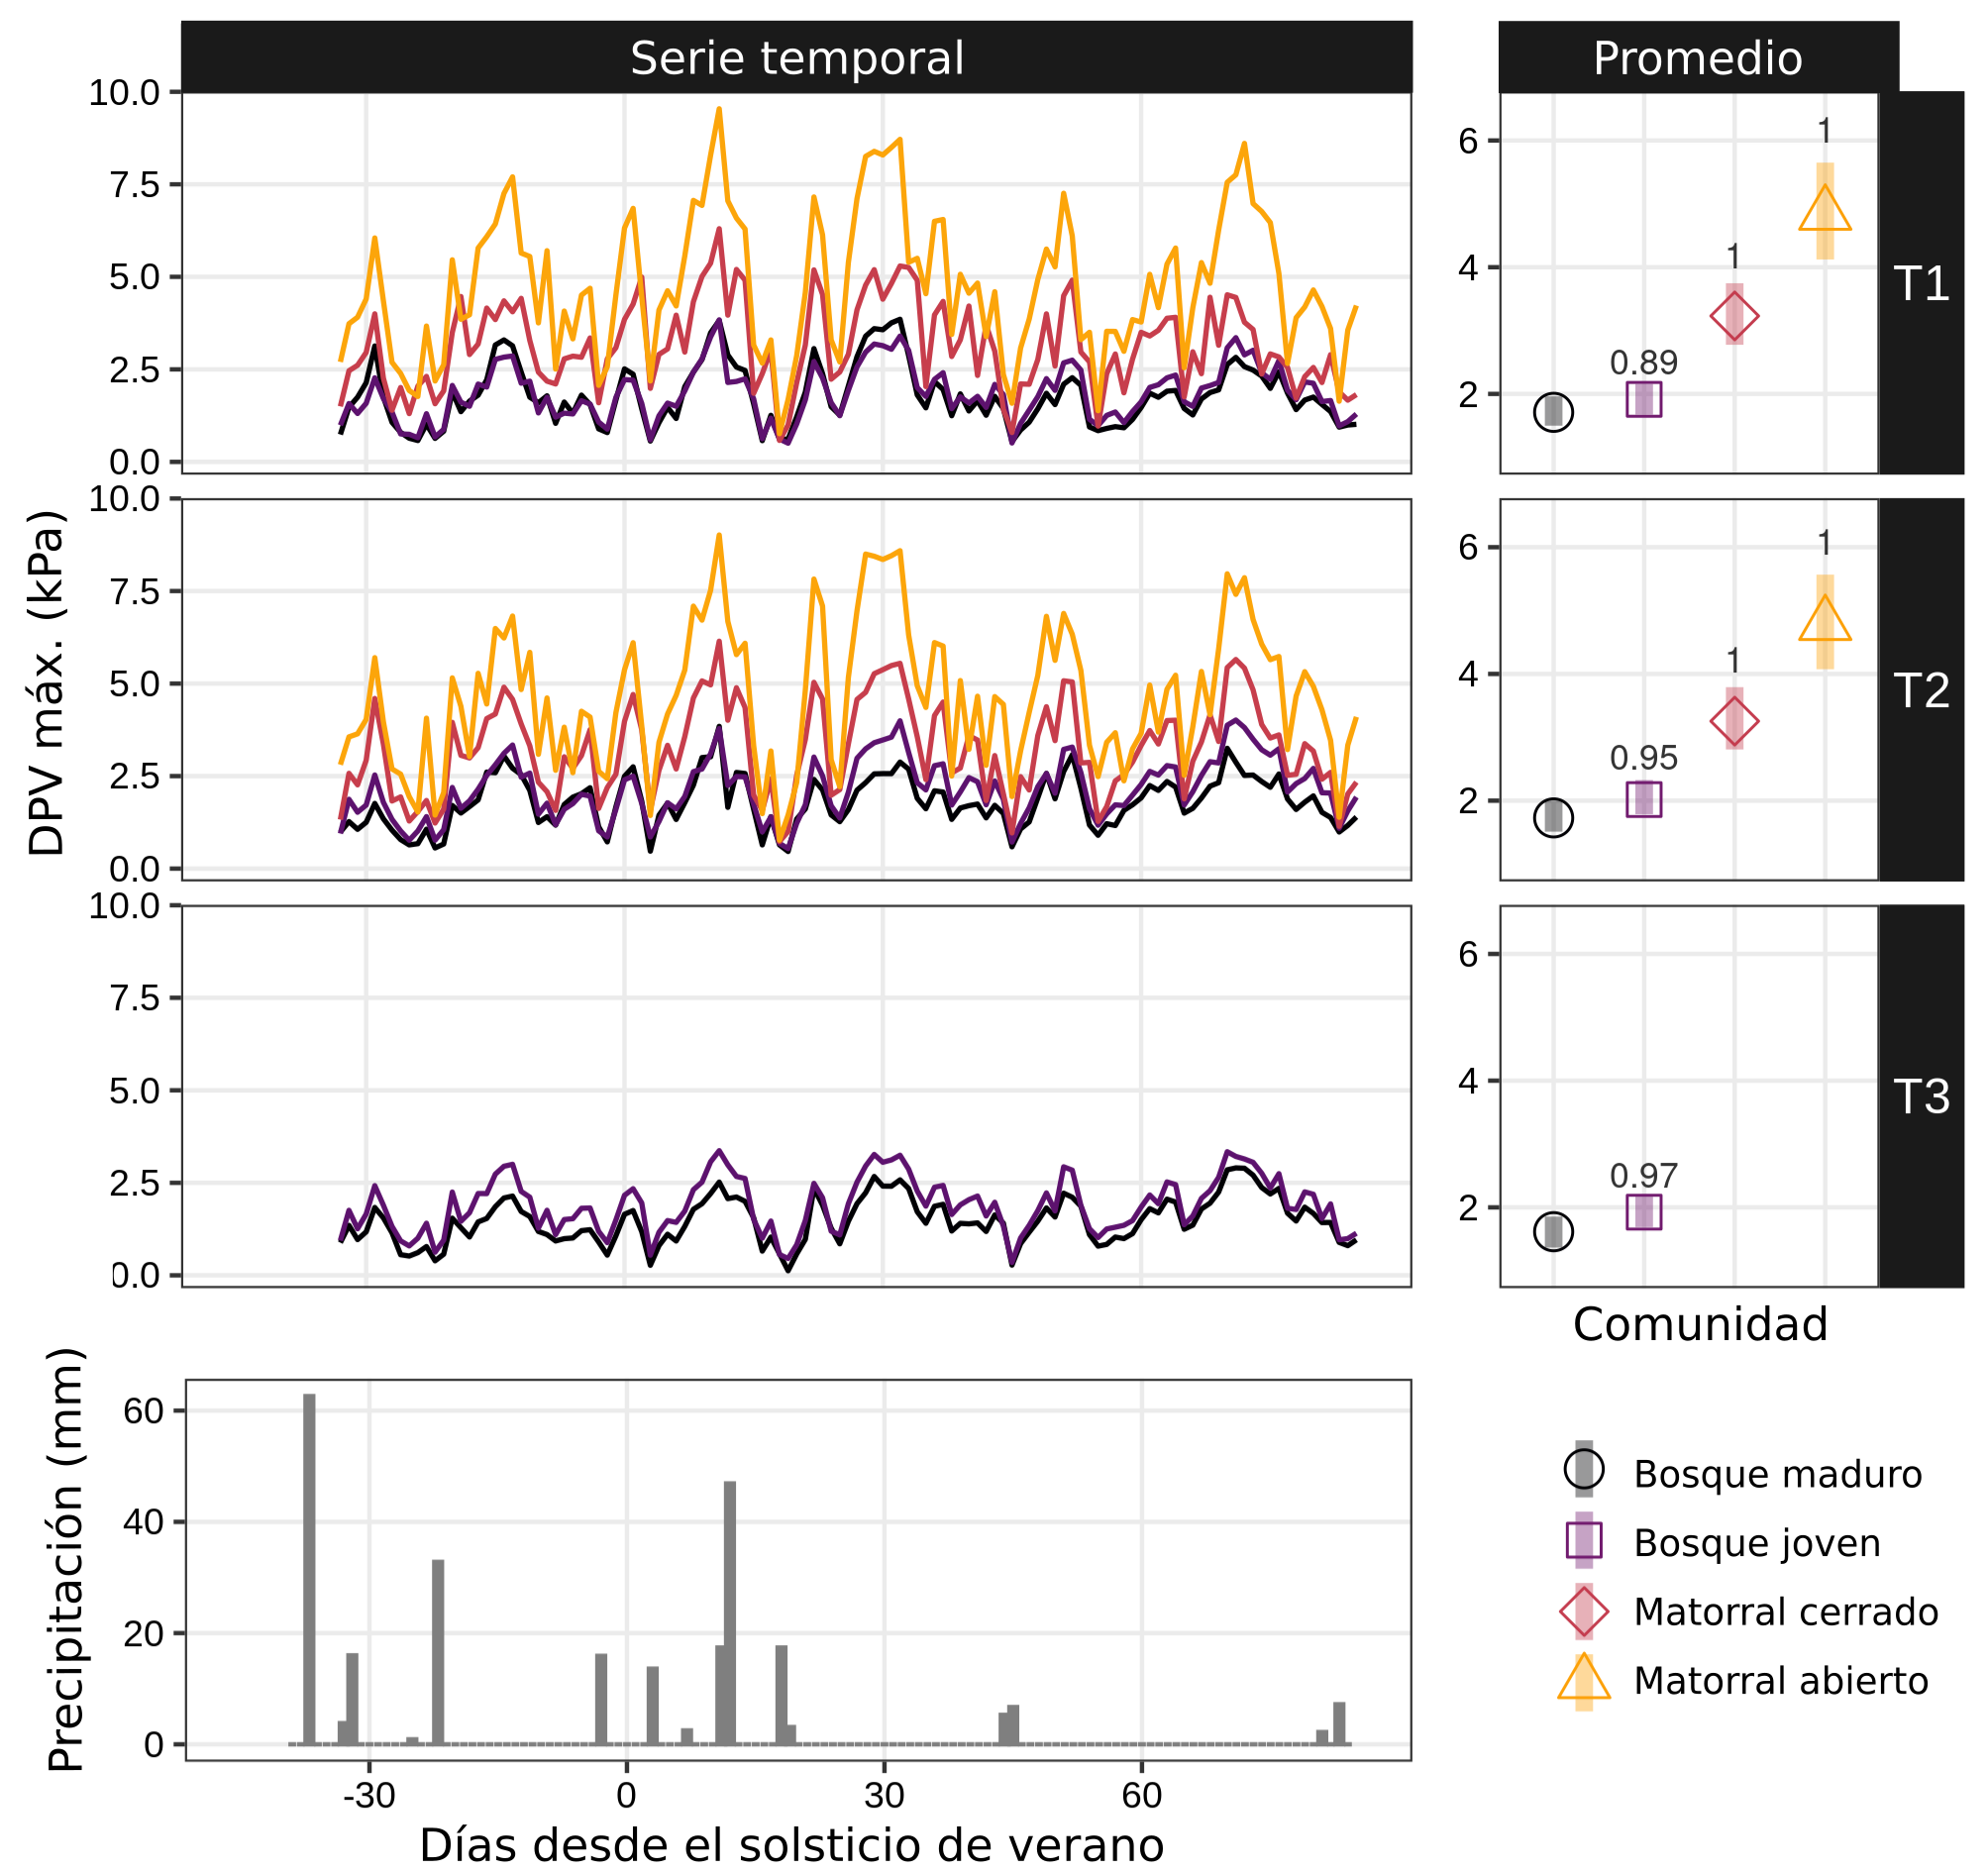
\includegraphics[width=16cm]{figuras/cap2/02) microclimate.png}
    \caption[Variación del microclima entre comunidades.]{Series temporales del Déficit de Presión de Vapor (DPV) máximo diario por comunidad y transecta (T), medido a $\approx$~50 cm sobre el suelo (paneles izquierdos). El día cero corresponde al 21 de diciembre de 2019. El panel inferior izquierdo muestra la precipitación diaria registrada en una estación meteorológica ubicada a 6 km del área de estudio. Los paneles derechos muestran el promedio estimado de DPV máximo por sitio (medias e intervalos de credibilidad del 95 \% de la distribución posterior), los cuales coinciden con los promedios observados. Los números sobre las barras indican la probabilidad posterior de que el promedio de DPV máximo en cada comunidad sea mayor que en el bosque maduro en su correspondiente transecta, estimada con el modelo de DPV. Los valores de probabilidad cercanos a 1 indican que una comunidad dada tiene un DPV mayor que el bosque maduro en su transecta (esperado), 0.5 indica que no hay diferencias, y valores cercanos a 0 indican un DPV mayor en el bosque maduro (no esperado).} 
    \label{fig:cap2-02}
\end{figure}

\subsection{Humedad del combustible}

\subsubsection{Combustibles muertos}

El contenido de humedad de la hojarasca (mezcla de combustibles) y el de las varillas de combustible (combustibles de composición similar) variaron entre comunidades de manera similar, pero de manera opuesta al DPV, siendo más bajo en los matorrales y mostrando una diferencia menor y más variable entre bosques jóvenes y maduros. Los matorrales abiertos presentaron un contenido de humedad ligeramente menor que los matorrales cerrados (Fig.~\ref{fig:cap2-03}a–\ref{fig:cap2-03}c). El contenido de humedad promedio por sitio mostró una relación negativa con el DPV máximo promedio del sitio (Fig.~\ref{fig:cap2-04}a–\ref{fig:cap2-04}c). El contenido de humedad de la hojarasca mostró mayor variabilidad que el de las varillas de combustible a todos los niveles (entre sitios, fechas y parcelas; Fig.~\ref{fig:cap2-03}a–\ref{fig:cap2-03}c y \ref{fig:cap2-S10}–\ref{fig:cap2-S12}).

\subsubsection{Combustibles vivos}

Los combustibles vivos de una sola especie (composición similar) mostraron un mayor contenido de humedad en los bosques maduros, con una relación negativa respecto al DPV, aunque esta relación no fue clara para todas las especies. En \textit{S. patagonicus}, este patrón fue consistente entre transectas, y el contenido de humedad mostró una clara relación negativa con el DPV (Fig.~\ref{fig:cap2-03}d y \ref{fig:cap2-04}d). En \textit{S. patagonicus}, al igual que en los combustibles muertos, los bosques jóvenes mostraron un contenido de humedad ligeramente menor que los bosques maduros, mientras que los matorrales presentaron valores mucho más bajos (Fig.~\ref{fig:cap2-03}d).

En \textit{N. dombeyi} y \textit{C. culeou}, las diferencias en el contenido de humedad entre comunidades fueron menores (Fig.~\ref{fig:cap2-03}e y \ref{fig:cap2-03}f). Para \textit{N. dombeyi}, el efecto del DPV fue despreciable, aunque con una tendencia negativa (Fig.~\ref{fig:cap2-04}e), y para \textit{C. culeou} encontramos un efecto negativo débil, pero su estimación fue bastante incierta debido al bajo número de sitios donde esta especie estuvo presente (Fig.~\ref{fig:cap2-04}f).

El contenido de humedad de la mezcla de combustibles vivos fue, en promedio, más alto en los matorrales, pero las diferencias entre comunidades variaron entre transectas: en la transecta 1, los matorrales abiertos y cerrados mostraron un mayor contenido de humedad que el bosque maduro, mientras que en la transecta 2 estas comunidades mostraron valores similares. Los bosques jóvenes tuvieron un menor contenido de humedad que los bosques maduros en las transectas 1 y 2, pero se observó lo contrario en la transecta 3 (Fig.~\ref{fig:cap2-03}g). En la transecta 1, los valores más altos de contenido de humedad se observaron al inicio del verano, y las comunidades mostraron valores más similares hacia el final (Fig. \ref{fig:cap2-S16}).

El contenido de humedad de la mezcla de combustibles vivos mostró una relación positiva con el DPV (Fig.~\ref{fig:cap2-04}g). El ordenamiento de los sitios con respecto a la composición de especies que conforman el combustibles vivo mostró que el eje principal de variación (eje 1, Fig.~\ref{fig:cap2-05}) estaba correlacionado con el contenido de humedad promedio (coeficiente de correlación de Pearson = -0.81), lo que indica que el contenido de humedad está asociado a la composición de especies.

\begin{figure}[htbp]
    \centering
    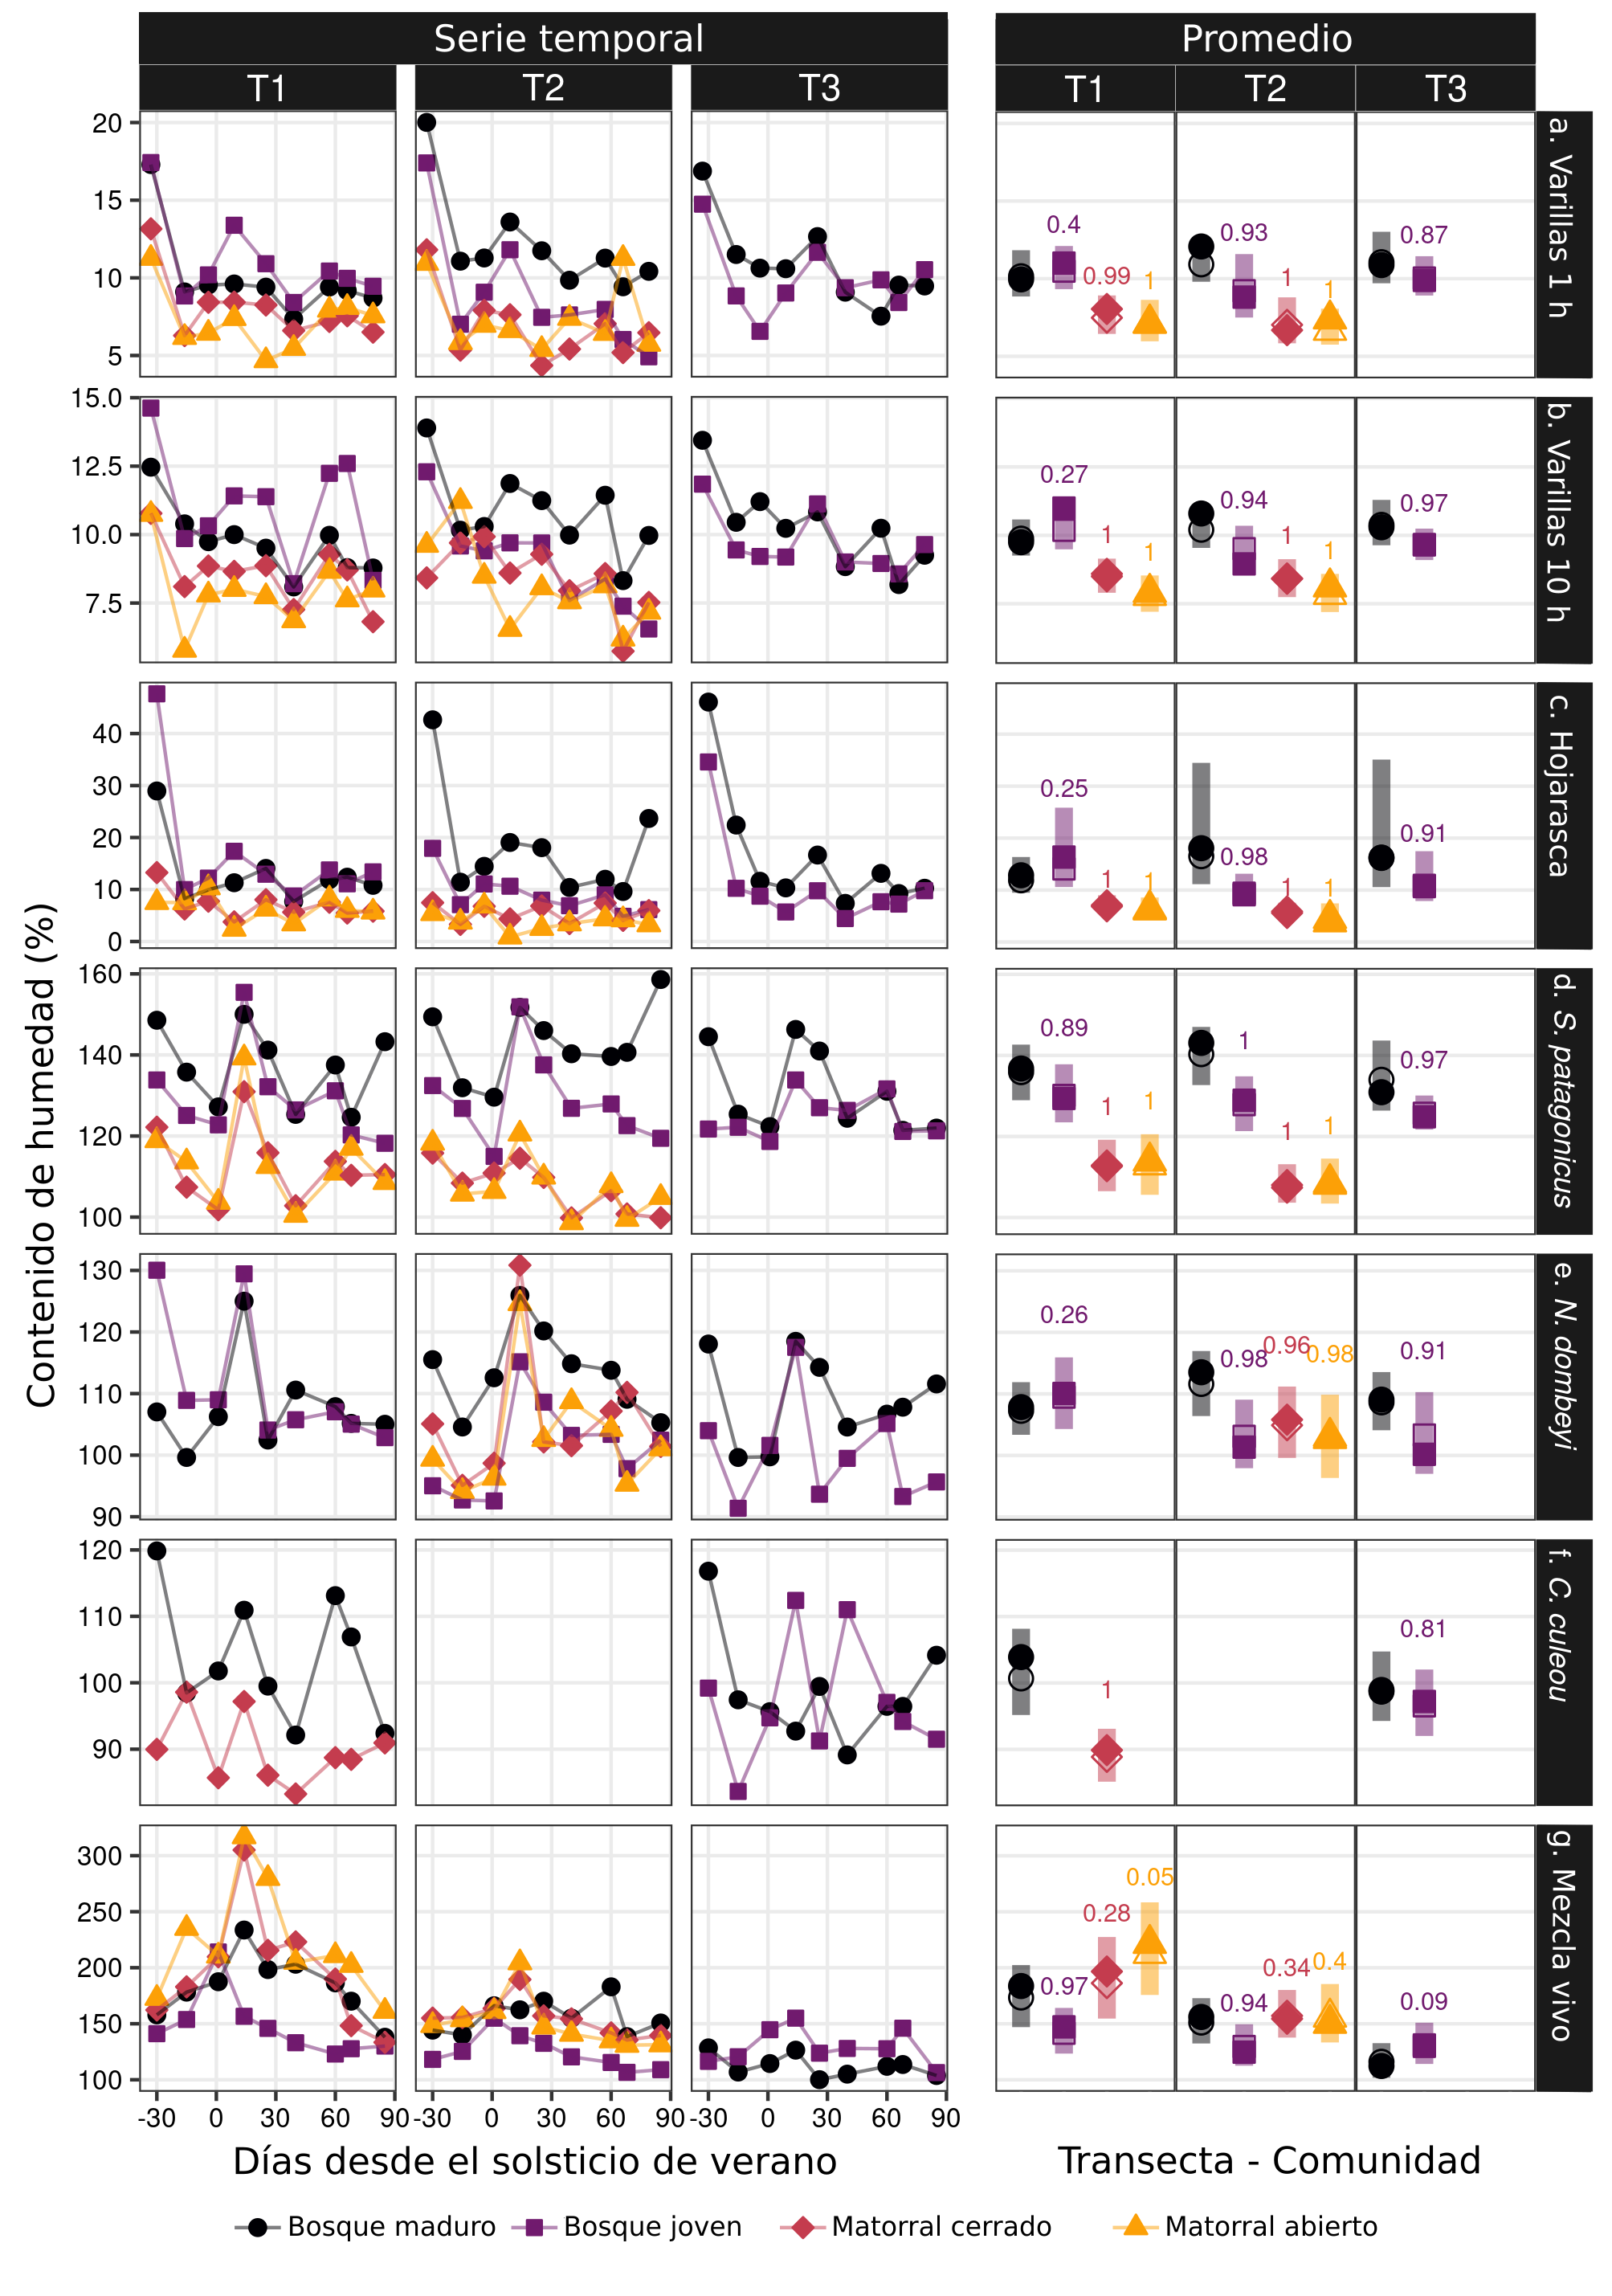
\includegraphics[width=15cm]{figuras/cap2/03) moisture ts.png}
    \caption[Variación del contenido de humedad del combustible entre comunidades.]{(Leyenda en la página siguiente.)}
    \label{fig:cap2-03}
\end{figure}

% leyenda en la página siguiente
\begin{figure}[p]
  \contcaption{(en la página anterior). Contenido de humedad del combustible por tipo de combustible, comunidad y transecta. Los valores para todas las fechas de muestreo se muestran en los paneles izquierdos, y los promedios de la temporada se presentan en los paneles derechos. El día cero corresponde al 21 de diciembre de 2019. En los paneles derechos, los símbolos abiertos y las barras muestran la media y el intervalo de credibilidad del 95 \% de la distribución posterior para el contenido de humedad promedio en cada sitio, estimados por los GLMMs, mientras que los símbolos llenos muestran las medias observadas. Los números sobre las barras indican la probabilidad posterior de que el contenido de humedad promedio en cada comunidad sea menor que en el bosque maduro de su correspondiente transecta. Los valores cercanos a 1 indican que una comunidad dada tiene un menor contenido de humedad que el bosque maduro en su transecta (esperado), 0.5 indica que no hay diferencias, y valores cercanos a 0 indican un menor contenido de humedad en el bosque maduro (no esperado).}
\end{figure}

\begin{figure}[htbp]
    \centering
    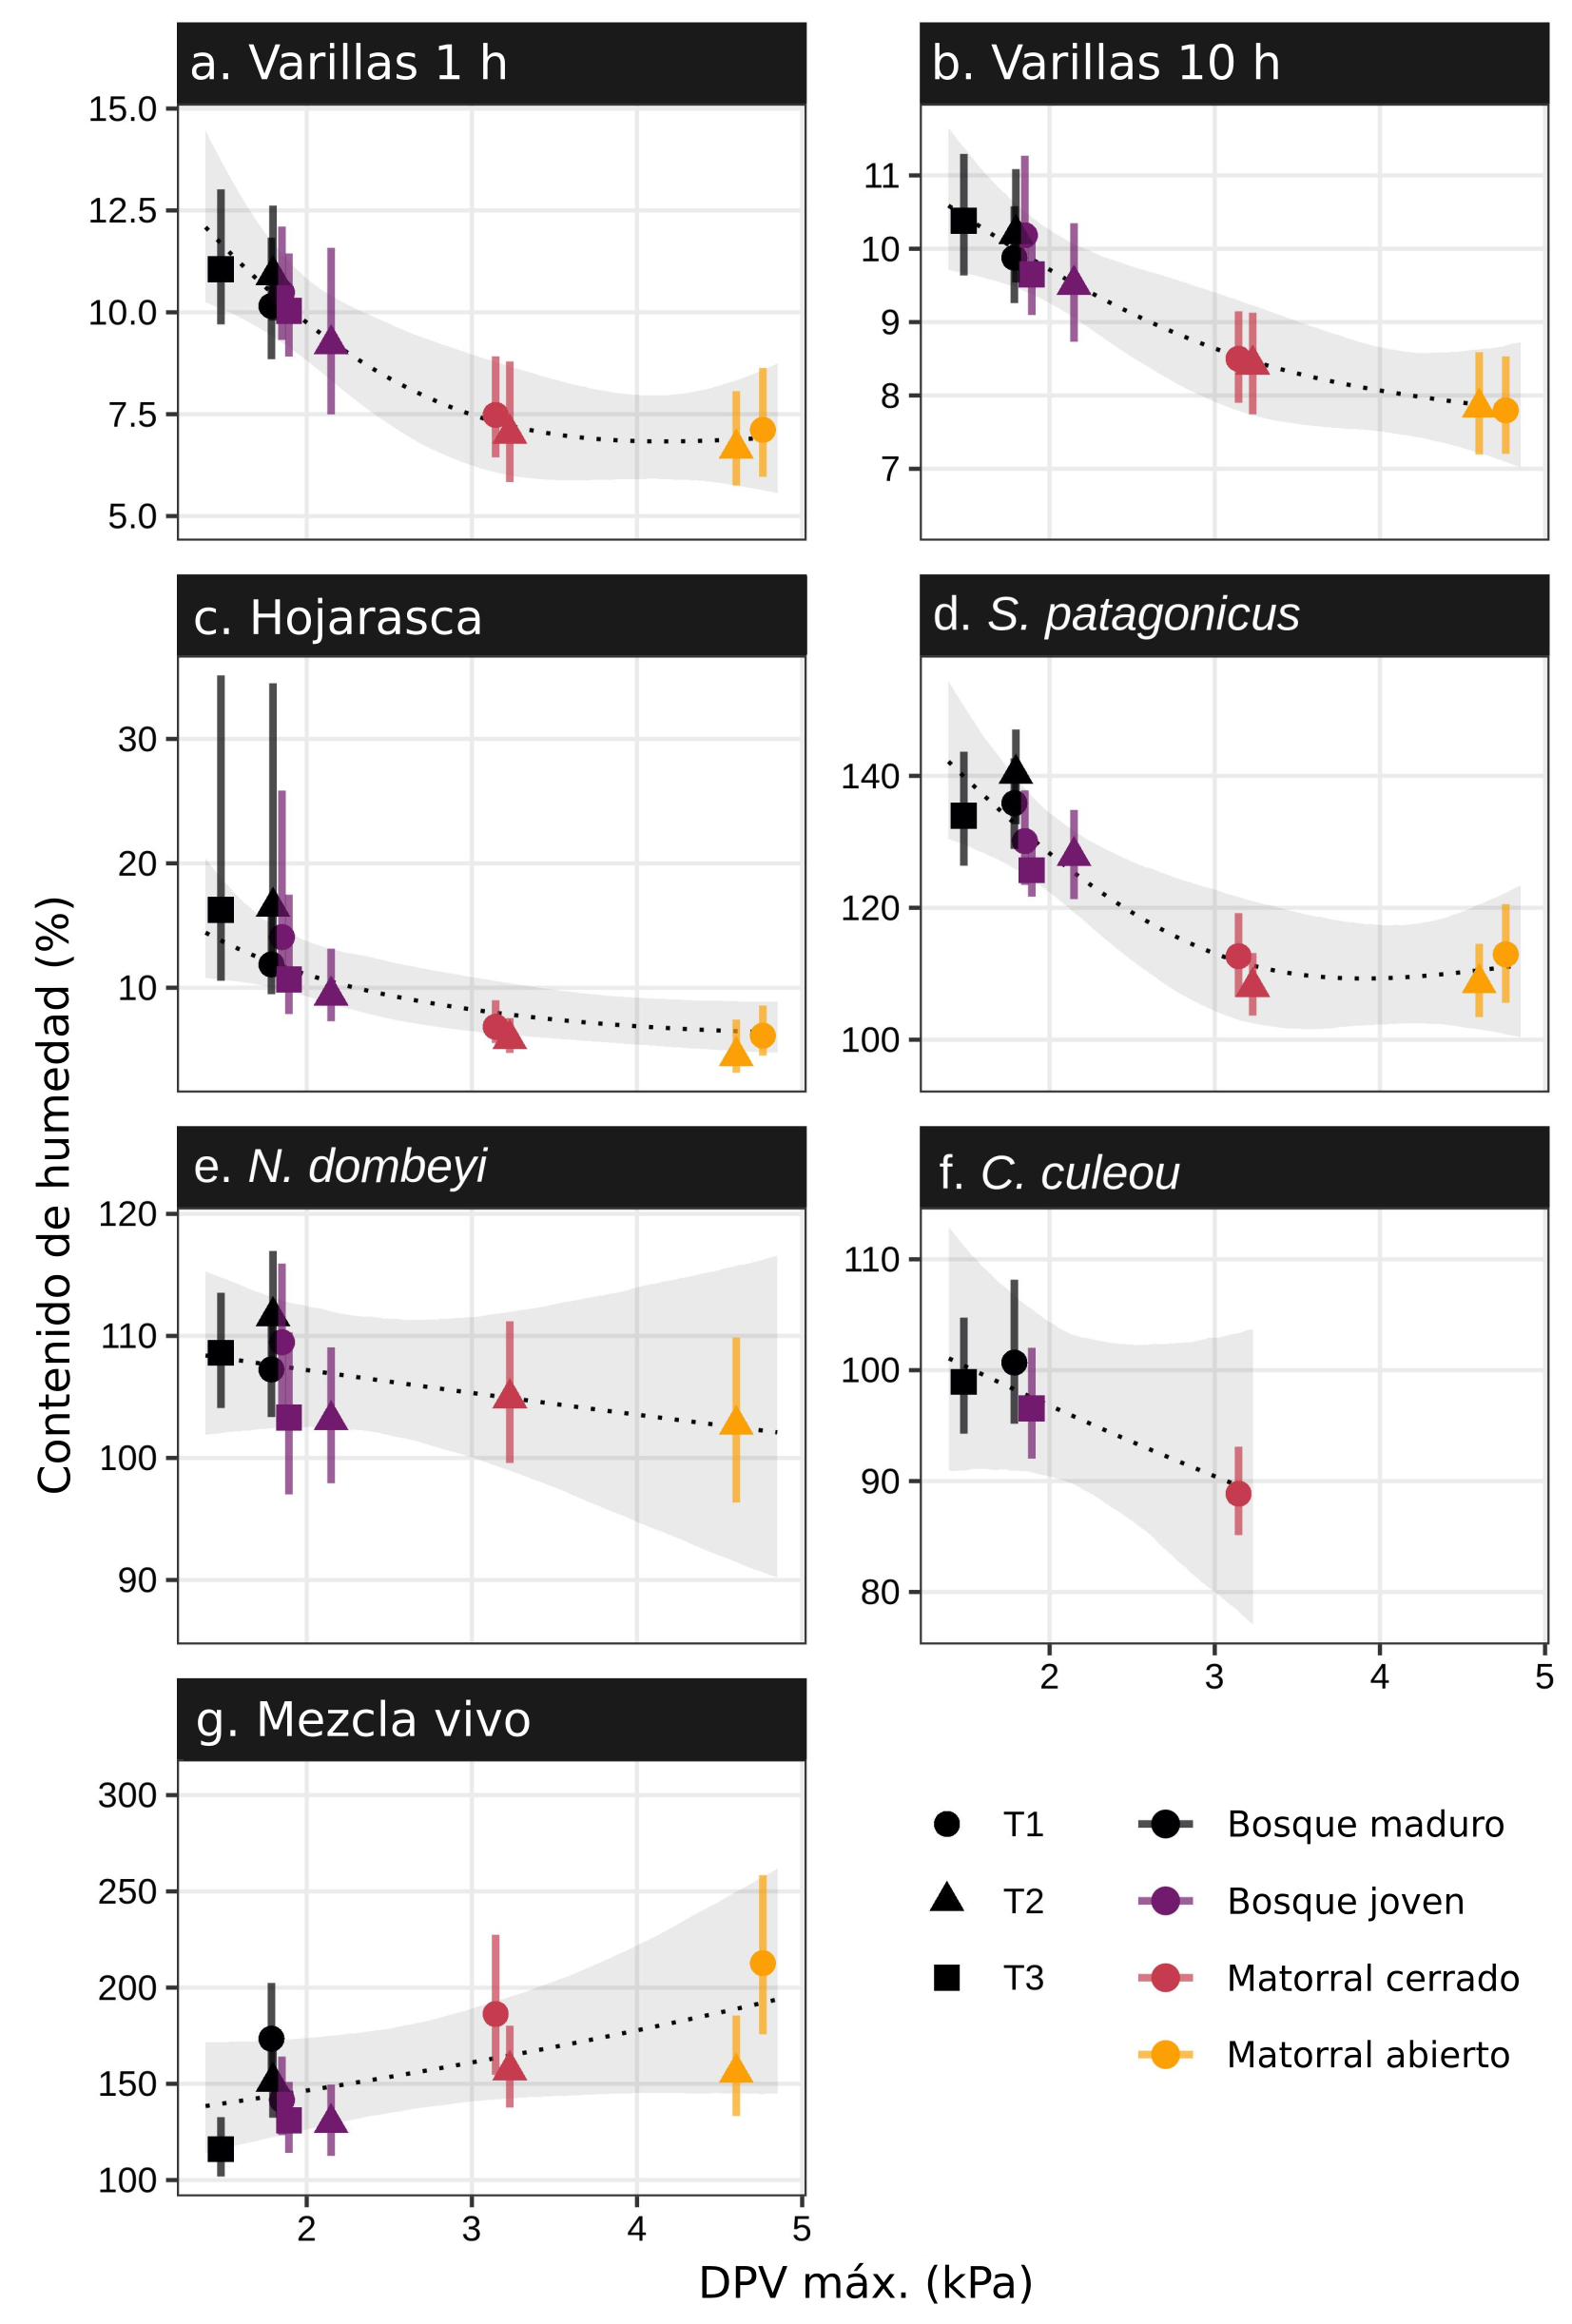
\includegraphics[width=13cm]{figuras/cap2/04) humedad - vpd.png}
    \caption[Contenido de humedad del combustible en función del Déficit de Presión de Vapor.]{Contenido de humedad promedio estimado en función del DPV máximo promedio por sitio. Los puntos representan la media de la distribución posterior para cada sitio, y las barras, los intervalos de credibilidad del 95 \% (mismos valores que en el panel derecho de la Fig.\ref{fig:cap2-03}). El efecto estimado del DPV se muestra con la línea punteada (media de la posterior) y la banda gris (IC del 95 \%).} 
    \label{fig:cap2-04}
\end{figure}

\begin{figure}[htbp]
    \centering
    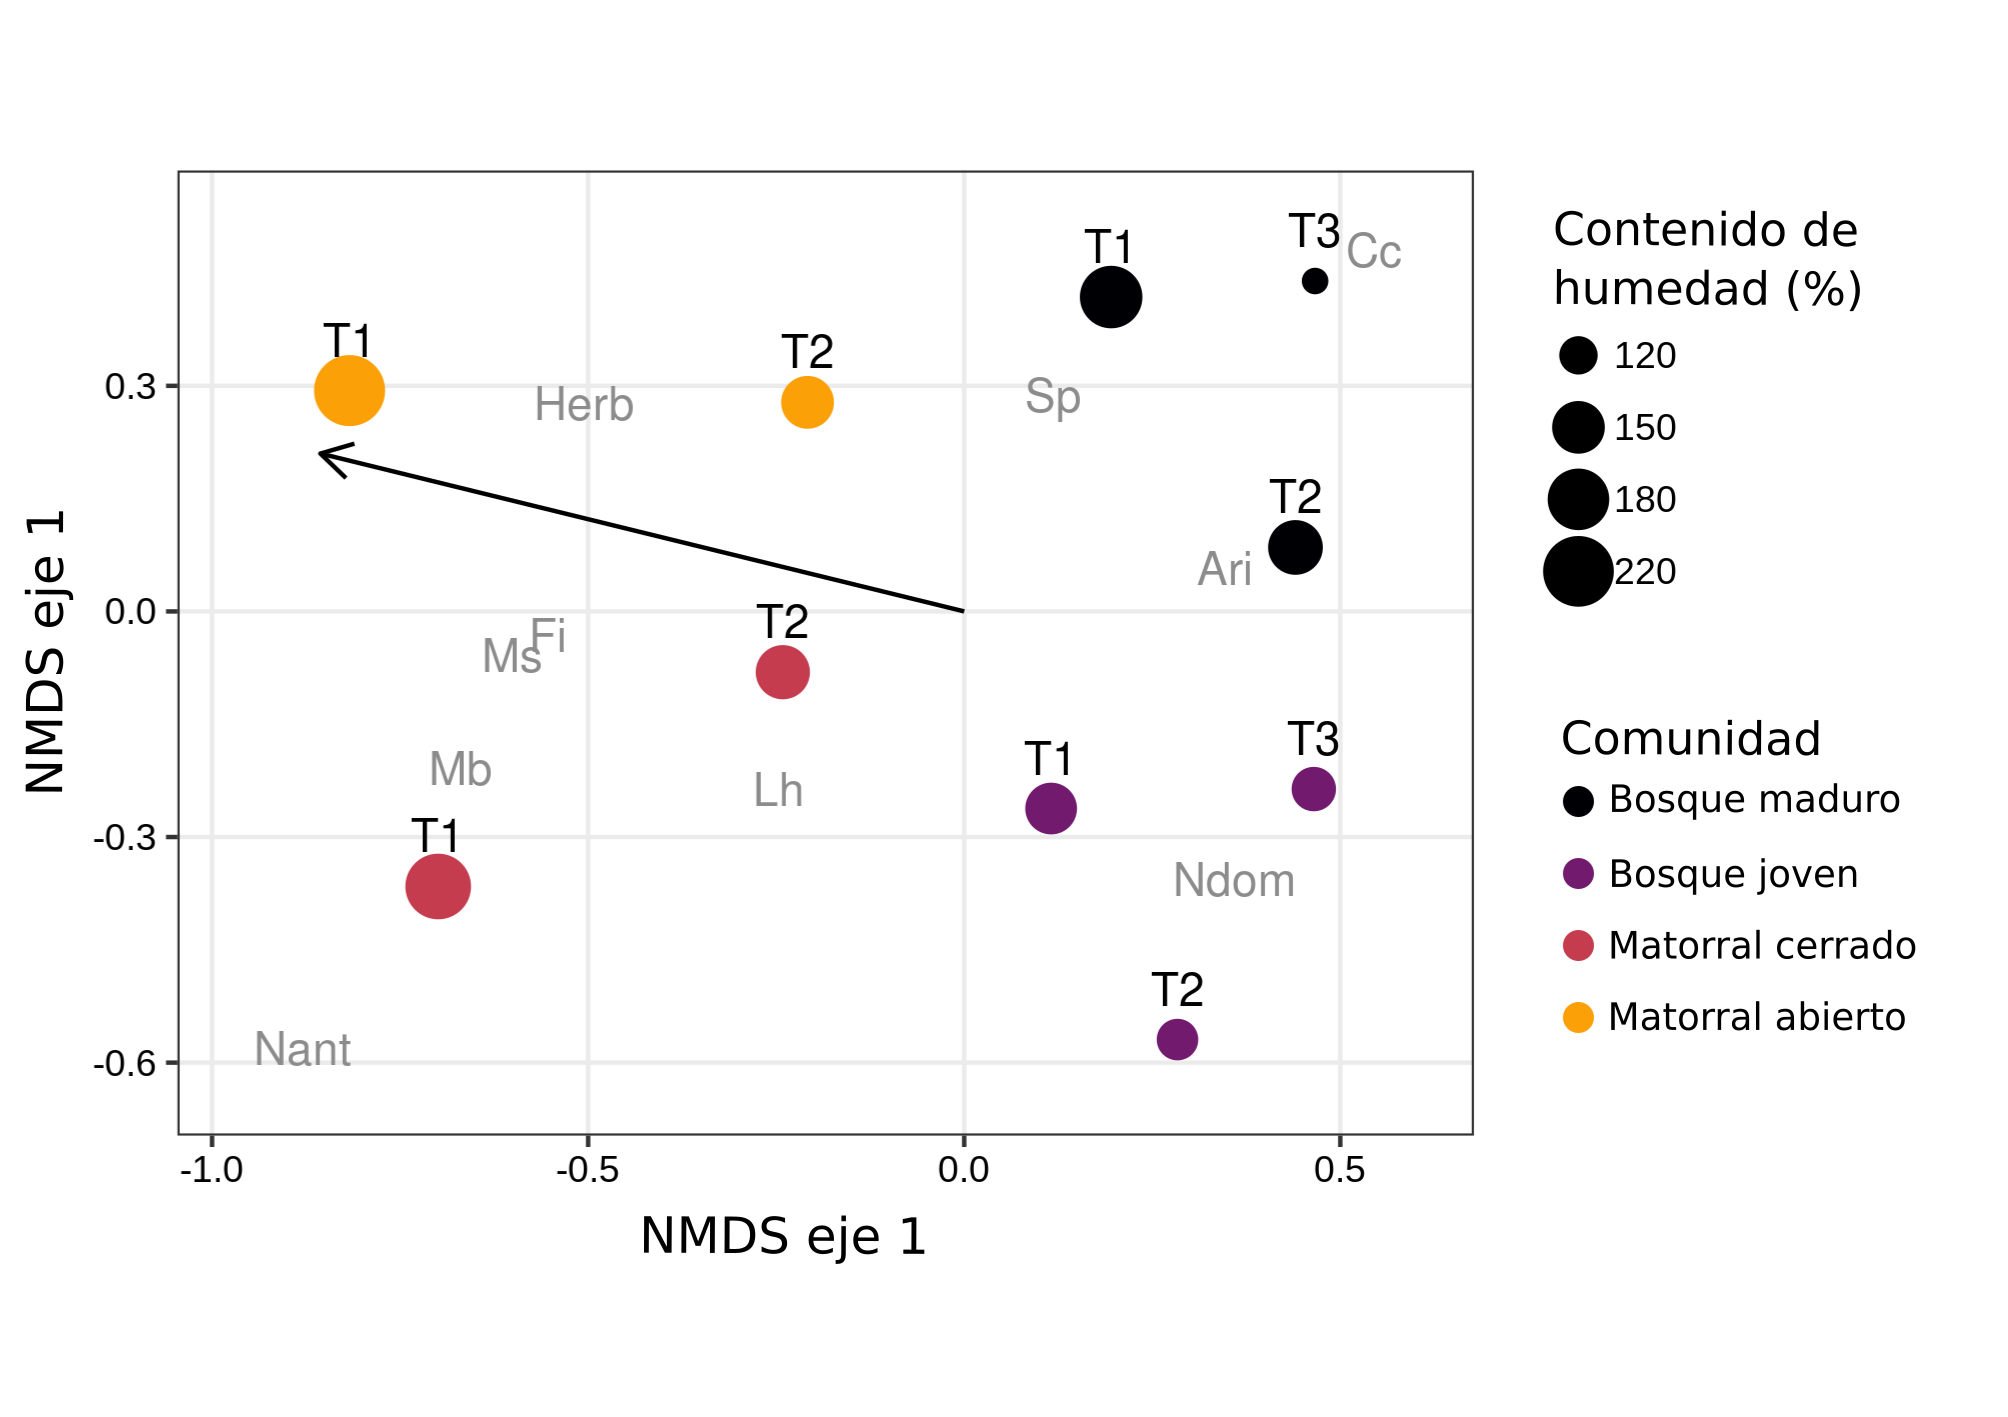
\includegraphics[width=15cm]{figuras/cap2/05) ordination.png}
    \caption[Ordenamiento de sitios según la composición de especies.]{Ordenamiento de sitios según la composición y abundancia de especies. Escalamiento Multidimensional No Métrico (NMDS) calculado a partir de los datos de intersección con varilla considerando solo combustibles vivos (\textit{stress} = 0.079; $\text{R}^2 \ \text{lineal} = 0.958$). Los sitios más cercanos en el gráfico son aquellos con una mayor similitud en la abundancia relativa de especies. Las coordenadas de la punta de la flecha muestran el coeficiente de correlación de Pearson entre los ejes y el contenido de humedad promedio de la mezcla de combustibles vivos por sitio (representado por el tamaño de los puntos). El texto en negro identifica las transectas, y el texto en gris, las coordenadas de las 10 especies más abundantes (Ndom: \textit{Nothofagus dombeyi}, Herb: especies herbáceas, Sp: \textit{Schinus patagonicus}, Cc: \textit{Chusquea culeou}, Ms: \textit{Mutisia spinosa}, Lh: \textit{Lomatia hirsuta}, Fi: \textit{Fabiana imbricata}, Ari: \textit{Aristotelia chilensis}, Nant: \textit{Nothofagus antarctica}, Mb: \textit{Maytenus boaria}).} 
    \label{fig:cap2-05}
\end{figure}

\FloatBarrier

\subsection{Probabilidad de ignición y disponibilidad del combustible}

Las diferencias en el contenido de humedad del combustible entre comunidades tuvieron un efecto claro en la probabilidad de ignición media, tanto para la hojarasca como para la mezcla de combustibles vivos. Para la hojarasca, la probabilidad de ignición en los bosques maduros estuvo mayormente por debajo de 0.9, mientras que en las demás comunidades tendió a ser más alta. En particular, los matorrales mostraron probabilidades de ignición superiores a 0.97 (Fig.~\ref{fig:cap2-06}, paneles superiores).

La probabilidad de ignición de la mezcla de combustibles vivos mostró un patrón variable entre transectas, al igual que su contenido de humedad. Los bosques jóvenes presentaron la mayor probabilidad de ignición, excepto en la transecta 3, donde fue mayor en el bosque maduro. Los matorrales mostraron una probabilidad de ignición menor que el bosque maduro en la transecta 1, y valores similares en la transecta 2 (Fig.~\ref{fig:cap2-06}, paneles inferiores).

La disponibilidad de combustible para la hojarasca mostró grandes diferencias entre comunidades, especialmente cuando se consideró el umbral de humedad para peligro de incendios extremo ($\le 9.85$ \%). En los bosques maduros, la humedad de la hojarasca cayó por debajo del umbral de 9.85 \% en solo 1 o 2 fechas de 9. En cambio, el contenido de humedad de los matorrales (abiertos o cerrados) estuvo por debajo de este umbral en la mitad o más de las fechas (Tabla~\ref{tab:fuel-availability}). Los bosques jóvenes mostraron una situación intermedia, cayendo por debajo del umbral crítico con mayor frecuencia que los bosques maduros, pero menor que los matorrales.

Todas las comunidades mostraron un contenido de humedad promedio de la hojarasca por debajo del umbral superior ($< 23.75$ \%) durante casi todas las fechas (8 o 9 de 9). Solo el 11 \% de las fechas mostraron simultáneamente humedad de la hojarasca en los matorrales $\le 9.85$ \%
y en los bosques maduros $> 23.75$ \% (Tabla~\ref{tab:fuel-availability}). Finalmente, el contenido de humedad promedio de la mezcla de combustibles vivos muy raramente cayó por debajo del 110 \%, con una tendencia a que esta condición ocurriera con mayor frecuencia en bosques maduros y jóvenes que en matorrales (Tabla~\ref{tab:fuel-availability}).

\begin{figure}[htbp]
    \centering
    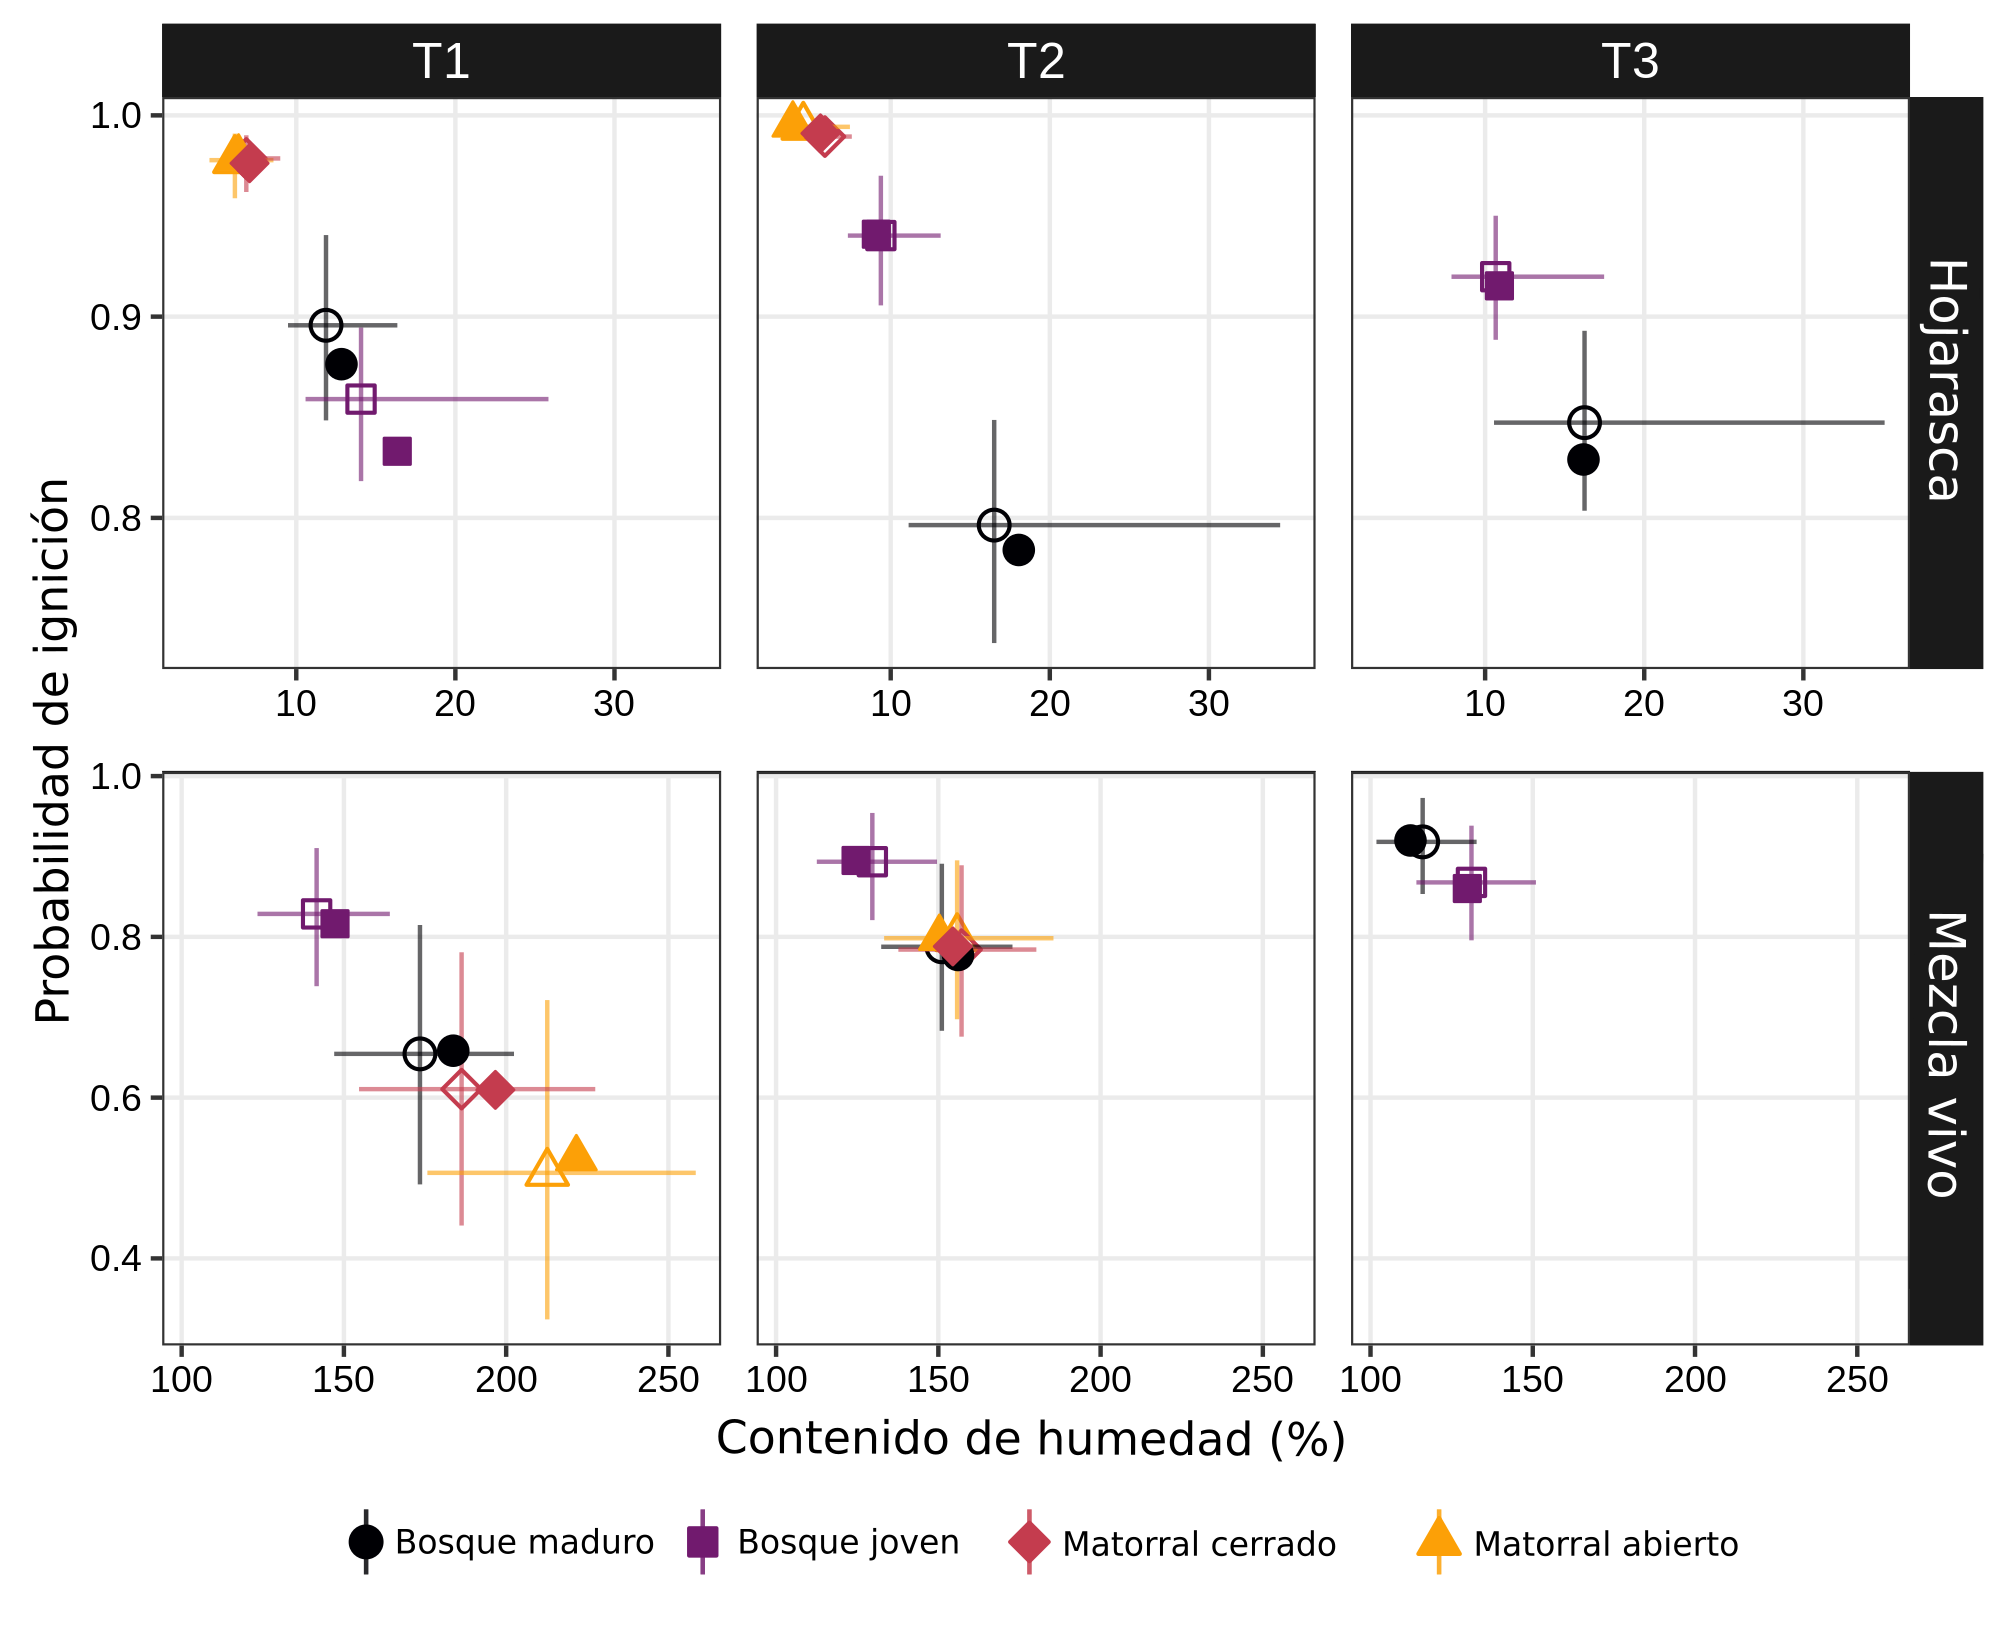
\includegraphics[width=16cm]{figuras/cap2/06) ig probability.png}
    \caption[Probabilidad de ignición.]{Probabilidad de ignición en función del contenido de humedad por comunidad, transecta y tipo de combustible. Los símbolos sólidos muestran la probabilidad de ignición y los promedios de contenido de humedad del combustible basados en los datos observados. Los símbolos abiertos y las barras muestran la media de la distribución posterior y los intervalos de mayor densidad del 95 \% basados en los valores de contenido de humedad del combustible simulados con los GLMMs.} 
    \label{fig:cap2-06}
\end{figure}

\begin{table}[ht]
\centering
\caption[Comparación de la disponibilidad de combustibles entre comunidades]{Comparación de la disponibilidad de combustibles entre comunidades. La disponibilidad de combustibles es el porcentaje de fechas (n = 9) en las que el contenido de humedad (CH) promedio estuvo por debajo de los umbrales críticos de peligro de incendios. Los umbrales de contenido de humedad de la hojarasca, 23.75 \% y 9.85 \%, son valores por debajo de los cuales la probabilidad de ignición de la hojarasca excede 0.5 y 0.98, respectivamente, según pruebas de ignición en laboratorio de \citet{bianchi_ignition_2014}. El umbral del 110 \% para la mezcla de combustibles vivos representa el contenido de humedad por debajo del cual se ha reportado la ocurrencia de incendios de gran magnitud en este sistema y otros similares \citep{chuvieco_prediction_2009, bianchi_live_2015, arganaraz_determining_2018}.}
\label{tab:fuel-availability}
\resizebox{16cm}{!}{%
\begin{tabular}{llccccc}
\toprule
\makecell{Tipo de\\combustible} & \makecell[c]{Umbral / comparación} & Transecta & \makecell{Bosque\\maduro} & \makecell{Bosque\\joven} & \makecell{Matorral\\cerrado} & \makecell{Matorral\\abierto} \\
\midrule
\multirow{9}{*}{Hojarasca} & \multirow{3}{*}{CH $\le$ 23.75 \%} & T1 & 88.89 & 88.89 & 100 & 100 \\
                        &  & T2 & 88.89 & 100 & 100 & 100 \\
                        &  & T3 & 88.89 & 88.89 & - & - \\
                        \cline{2-7}
                        & \multirow{3}{*}{CH $\le$ 9.85 \%} & T1 & 22.22 & 11.11 & 88.89 & 88.89 \\
                        & & T2 & 11.11 & 66.67 & 100 & 100 \\
                        & & T3 & 22.22 & 77.78 & - & - \\
                        \cline{2-7}
                        & \multirow{3}{*}{\makecell[l]{CH $>$ 23.75 \% en bosque maduro\\y $\le$ 9.85 \% en las demás}} & T1 & - & 0 & 0 & 11.11 \\
                        & & T2 & - & 0 & 11.11 & 11.11 \\
                        & & T3 & - & 0 & - & - \\
                        \cline{2-7}
\multirow{3}{*}{\makecell[l]{Mezcla de\\combustible vivo}} & \multirow{3}{*}{CH $\le$ 110 \%} & T1 & 0 & 0 & 0 & 0 \\
                                   & & T2 & 0 & 22.22 & 0 & 0 \\
                                   & & T3 & 44.44 & 11.11 & - & - \\
\bottomrule
\end{tabular}%
}
\end{table}

\FloatBarrier

\section{Discusión}

\subsection{Microclima}

Como se esperaba, encontramos un DPV máximo y una temperatura del aire más altos, junto con una humedad relativa mínima más baja en los sitios más abiertos en comparación con los bosques maduros. Esto concuerda con un estudio previo en bosques subalpinos de \textit{N. pumilio} \citep{paritsis_positive_2015} y con otros estudios en bosques templados y tropicales \citep{uhl_fire_1988, little_fire_2012, hoffmann_fuels_2012, jucker_canopy_2018, de_frenne_global_2019, kane_stand_2021, wolf_wildfire_2021}. Por el contrario, \citet{burton_shifting_2019} reportaron variaciones muy pequeñas en estas variables entre estados alternativos en bosques templados del sureste de Australia. Una posible razón para esta discrepancia podría ser que sus comunidades quemadas más recientemente tenían vegetación alta (10-15 m) y densa, probablemente albergando un microclima relativamente más fresco y húmedo que nuestros matorrales (con 1 a 4 m de altura).

Encontramos que los bosques jóvenes mostraron extremos de DPV, temperatura y humedad relativa similares a los bosques maduros. Esto podría explicarse por su alta densidad de vegetación desde el suelo hasta los 4 m de altura, que fue mucho menor en los matorrales cerrados y abiertos (Fig.~\ref{fig:cap2-S02} y \ref{fig:cap2-S03}). Sin embargo, las diferencias microclimáticas entre comunidades podrían variar si se consideran otras alturas \citep{pickering_darker_2021}. Por ejemplo, los bosques jóvenes, al carecer de un dosel alto, presentan menor cobertura de vegetación que los bosques maduros por encima de 1.5 m de altura (en lugar de 0.5 m, donde se instalaron los sensores; Fig.~\ref{fig:cap2-S04}). Por lo tanto, el DPV a 1.5 m probablemente sería más alto en los bosques jóvenes que en los maduros.

\subsection{Variación del contenido de humedad entre comunidades y su relación con el DPV}

Como esperábamos, el contenido de humedad de los combustibles muertos mostró una relación negativa con el DPV, probablemente reflejando el efecto del microclima sobre la tasa de evaporación, en concordancia con estudios previos \citep{uhl_fire_1988, hoffmann_fuels_2012, little_fire_2012, balch_susceptibility_2015, kane_stand_2021}. Nuestros resultados son consistentes con \citet{brown_sensitivity_2022}, quienes encontraron que el DPV en el sotobosque fue una de las variables microclimáticas más importantes controlando el contenido de humedad de varillas de combustible de 10 h en bosques templados del sureste de Australia. Sin embargo, dado que la estructura de la vegetación controla también otras variables microclimáticas, es probable que los sitios más abiertos (e.g., matorrales) no solo muestren un DPV más alto, sino también mayor radiación solar y mayor velocidad del viento \citep{little_fire_2012, jucker_canopy_2018, de_frenne_global_2019, wolf_wildfire_2021}. Por lo tanto, el efecto del DPV que observamos sobre el contenido de humedad de combustibles muertos probablemente refleja un efecto compuesto de todas estas variables microclimáticas correlacionadas.

La estructura de la vegetación también podría explicar las similitudes observadas en el DPV y, consecuentemente, en el contenido de humedad de combustibles muertos entre bosques jóvenes y maduros. Este resultado concuerda parcialmente con \citet{brown_forest_2021}, quienes encontraron una relación positiva entre el contenido de humedad de las varillas de combustible de 10 h y la densidad de la vegetación entre 0.5 y 2 m de altura en bosques templados del sureste de Australia. Tanto las mezclas como los combustibles muertos de composición similar (hojarasca y varillas de combustible) mostraron la misma relación entre el contenido de humedad y el DPV, lo que sugiere que la composición de especies no ejerce un control importante sobre el contenido de humedad de la hojarasca. Sin embargo, la mayor variabilidad en el contenido de humedad de la hojarasca entre sitios, fechas y parcelas, en comparación con las varillas de combustible, podría explicarse parcialmente por la composición de la hojarasca.

En cuanto a los combustibles vivos, encontramos que un microclima más húmedo y fresco promueve un mayor contenido de humedad dentro de una misma especie, pero el patrón opuesto se observó a nivel comunitario. Los combustibles vivos de una sola especie tendieron a mostrar mayor contenido de humedad en los sitios más frescos y húmedos, particularmente en el arbusto \textit{S. patagonicus}. Los efectos microclimáticos estimados mostraron una considerable incertidumbre en el caso de \textit{C. culeou} y \textit{N. dombeyi}, probablemente debido al reducido número de sitios (cuatro y seis, comparado con los 10 de \textit{S. patagonicus}), aunque este patrón coincide con los resultados de \citet{blackhall_is_2012} para un mayor número de sitios y especies. Las autoras reportaron que las plantas en comunidades posfuego usualmente tienen rasgos foliares más inflamables (incluyendo menor contenido de humedad) en comparación con las mismas especies en sitios no quemados. Como se mencionó para los combustibles muertos, el efecto del DPV sobre el contenido de humedad de combustibles vivos de una sola especie probablemente refleja un efecto compuesto de otras variables microclimáticas correlacionadas, como la radiación y la velocidad del viento, que actuarían durante la etapa de desarrollo del tejido foliar \citep{aroca_plant_2012}.

El contenido de humedad a nivel comunitario (mezclas de combustibles vivos) mostró un patrón opuesto al de los combustibles vivos de una sola especie, siendo mayor o similar en los sitios más desecantes. Esto sugiere que el microclima afecta los rasgos de las plantas dentro de una especie, pero no necesariamente promueve la dominancia de especies esclerófilas en los sitios más desecantes. La relación positiva entre el DPV y el contenido de humedad de las mezclas de combustibles vivos está influenciada por los altos valores encontrados en los matorrales de la transecta 1, mientras que los matorrales de la transecta 2 mostraron valores similares a los de las otras comunidades. Estas variaciones podrían explicarse parcialmente por la composición y abundancia de especies. Por ejemplo, el bajo contenido de humedad en los bosques maduros y jóvenes probablemente esté relacionado con su alta abundancia de \textit{N. dombeyi} y \textit{C. culeou} (Tabla~\ref{tab:sp-composition} y Fig.~\ref{fig:cap2-S05}), especies cuyo contenido de humedad medio es bajo y muy bajo, respectivamente \citep{bianchi_comparison_2018, blackhall_flammability_2019}. Además, el bajo contenido de humedad en el bosque maduro de la transecta 3 podría explicarse por su alta abundancia relativa de \textit{C. culeou} ($\approx$~60 \%, Tabla~\ref{tab:sp-composition} y Fig.~\ref{fig:cap2-S05}). Por otro lado, la presencia de pastos y otras plantas herbáceas (como \textit{Vicia} sp., observada en los matorrales estudiados) podría aumentar el contenido de humedad en los matorrales.

También encontramos que en la transecta 1 la variabilidad en el contenido de humedad entre comunidades fue grande a mediados del verano, pero pequeña al inicio y final de la estación seca (Fig.~\ref{fig:cap2-S16}). Estas dinámicas estacionales suelen resultar de cambios no solo en el contenido de agua, sino también en el contenido de materia seca \citep{jolly_-coupling_2014, qi_spectroscopic_2014}. Algunas especies, como \textit{N. dombeyi}, \textit{N. antarctica}, o plantas herbáceas, producen follaje nuevo hacia fines de la primavera, aumentando su contenido de humedad, mientras que otras alcanzan su contenido máximo de humedad a principios o finales del verano, probablemente cuando producen nuevas hojas (e.g., \textit{Lomatia hirsuta}, \textit{Austrocedrus chilensis} y \textit{Maytenus boaria}; Kitzberger, datos no publicados). Los cambios en la humedad del suelo relacionados con la lluvia también podrían haber contribuido a estas variaciones temporales en el contenido de humedad de las mezclas de combustibles vivos, pero el hecho de que solo en la transecta 1 se haya observado un pico en el contenido de humedad vuelve esta explicación poco plausible.

\subsection{Contribución de la humedad del combustible a las diferencias de inflamabilidad}

Nuestros resultados sugieren que el contenido de humedad de la hojarasca contribuye a la diferencia de inflamabilidad entre comunidades pirófilas y pirófobas. El menor contenido de humedad en la hojarasca de los matorrales en comparación con los bosques maduros resultó en una mayor probabilidad de ignición y disponibilidad de combustible en los primeros. Al comparar bosques maduros y jóvenes, la diferencia en la probabilidad de ignición y disponibilidad de combustible fue menor, lo que sugiere que el contenido de humedad de la hojarasca presenta una contribución pequeña a su diferencia en inflamabilidad.

La contribución del contenido de humedad de la hojarasca a las diferencias de inflamabilidad entre comunidades depende de cómo la estructura de la vegetación sobre la hojarasca controla el microclima cercano a la superficie. Aunque los bosques jóvenes carecen de un dosel alto, su alta densidad de árboles y arbustos jóvenes, de alrededor de 4 m de altura, genera un microclima sombreado cerca de la superficie. Nuestros resultados se asemejan a patrones descritos en bosques templados de eucaliptos (sureste de Australia), donde la edad del rodal y la estructura del dosel por sí solas no explican las variaciones en el contenido de humedad de la hojarasca \citep{cawson_fuel_2017, burton_shifting_2019, brown_forest_2021}. Por ejemplo, \citet{cawson_fuel_2017} reportaron mayor contenido de humedad en combustibles muertos en comunidades con regeneración vigorosa tras un incendio severo en comparación con bosques antiguos más abiertos o bosques tras incendios de baja severidad, donde la regeneración era escasa. Contrariamente, \citet{burton_shifting_2019} encontraron que los bosques no quemados por largos períodos albergan un elevado contenido de humedad en combustibles muertos, asociado a una densa capa de helechos cerca de la superficie. En nuestro estudio, los matorrales jóvenes cerrados, eran, aparentemente, lo suficientemente abiertos como para que la hojarasca mostrara un menor contenido de humedad que en los bosques. Sin embargo, matorrales más antiguos, con mayor densidad y altura de combustibles \citep{paritsis_positive_2015, tiribelli_changes_2018}, probablemente alberguen una capa de hojarasca más húmeda. De esta forma, el contenido de humedad de la hojarasca probablemente contribuiría poco a la diferencia de inflamabilidad entre bosques maduros y matorrales maduros. Sin embargo, la hojarasca es solo un componente del combustible en los ecosistemas del norte de la Patagonia Andina, y otros tipos de combustible también deben ser considerados.

Dado que la cobertura de vegetación sobre los combustibles muertos parece controlar su contenido de humedad, se deberían esperar resultados diferentes para combustibles muertos elevados en comparación con la hojarasca. En comunidades de baja estatura ($\approx$~4 m) que carecen de un dosel alto y cerrado, el contenido de humedad de la biomasa muerta en pie probablemente disminuya en función de la altura, siendo las hojas y ramas muertas más altas probablemente tan susceptibles a la desecación como la hojarasca en los matorrales abiertos. Esto es relevante porque algunas especies abundantes en los matorrales, como \textit{Lomatia hirsuta}, \textit{N. antarctica}, \textit{C. culeou}, \textit{Diostea juncea} y \textit{Mutisia} sp., forman densos paquetes de combustible fino muerto en pie \citep{blackhall_is_2012}. Dado que la profundidad de la hojarasca suele ser somera en los ecosistemas del norte de la Patagonia Andina ($\approx$~2 cm; Fig.~\ref{fig:cap2-S04} y \citealt{blackhall_effects_2017}) y que el fuego se propaga tanto a través de la biomasa superficial como en pie \citep{zylstra_biophysical_2016, ziegler_spatially_2017}, es importante considerar tanto los combustibles muertos como los vivos en pie al evaluar las variaciones de inflamabilidad entre comunidades.

Nuestros resultados sugieren que la contribución del contenido de humedad de los combustibles vivos a las diferencias de inflamabilidad entre comunidades depende en gran medida de la composición de especies y no necesariamente del microclima. La probabilidad de ignición estimada para las mezclas de combustibles vivos mostró una alta variabilidad entre comunidades, sugiriendo que los bosques maduros y jóvenes son los más inflamables a nivel de muestra foliar, mientras que los matorrales mostraron probabilidades de ignición similares o menores, dependiendo de la transecta. Las únicas comunidades donde el contenido de humedad de las mezclas de combustibles vivos cayó por debajo del valor crítico de 110 \% fueron los bosques jóvenes y maduros. Esto muestra que, según la composición de especies, la humedad de los combustibles vivos podría influir en la inflamabilidad en el sentido contrario a la carga, la continuidad del combustible y la humedad de la hojarasca. Claramente, en este caso, la humedad de los combustibles vivos juega un papel secundario en la determinación del peligro de incendios, como lo demuestran los patrones de actividad del fuego (frecuencia, área quemada) en estas comunidades \citep{mermoz_landscape_2005, morales_stochastic_2015, paritsis_positive_2015, tiribelli_non-additive_2019}.

El rol secundario de la humedad del combustible vivo sobre la inflamabilidad podría explicarse por la interacción de diferentes propiedades del combustible a nivel de rodal para determinar el comportamiento del fuego \citep{fernandes_plant_2012, zylstra_biophysical_2016}. La ignición del follaje vivo depende fuertemente del calor liberado por otras partículas de combustible en combustión y de la distancia entre ellas \citep{zylstra_biophysical_2016}. De esta forma, aunque los combustibles vivos podrían estar más húmedos (y, por ende, menos inflamables a nivel de hoja) en los matorrales que en los bosques, la alta carga y continuidad de combustibles en los primeros probablemente aumenta su probabilidad de ignición al exponer las hojas a un mayor flujo de calor. Otros estudios también han encontrado patrones contrastantes al evaluar la inflamabilidad de elementos de combustible separados (e.g., hojas) y estructuras más complejas, como plantas completas o camas de combustible \citep{fernandes_plant_2012}. Esto resalta la necesidad de evaluar la inflamabilidad considerando todas las propiedades del combustible (calidad, incluyendo composición química, carga y disposición) de forma conjunta como lo proponen \citet{zylstra_biophysical_2016}. Otra posible causa de una mayor inflamabilidad de matorrales a pesar de su elevado contenido de humedad de combustible vivo es que las especies que los componen presenten una composición química foliar que otorgue mayor inflamabilidad. Compuestos como terpenos, resinas, o metabolitos secundarios volátiles pueden facilitar la ignición y la propagación del fuego \citep{alessio_influence_2008, guerrero_unraveling_2024}. Estudios futuros podrían considerar este aspecto de la calidad del combustible, además de su humedad, carga y disposición.

\section{Conclusiones}

Encontramos que los bosques pirófobos del norte de la Patagonia Andina presentan sotobosques más húmedos y frescos, con un mayor contenido de humedad en los combustibles muertos, en comparación con los matorrales pirófilos, lo que probablemente contribuye a su menor inflamabilidad \citep{mermoz_landscape_2005, morales_stochastic_2015, paritsis_positive_2015, tiribelli_non-additive_2019}, junto con la mayor carga y continuidad de combustibles previamente reportadas \citep{paritsis_positive_2015, tiribelli_changes_2018}. Los combustibles vivos mostraron un patrón similar en el contenido de humedad que los combustibles muertos cuando se consideraron las especies por separado, pero el contenido de humedad a nivel comunitario de las mezclas de combustibles vivos fue mayor en los matorrales pirófilos. Esto demuestra que los cambios en la composición de especies y su abundancia relativa pueden anular el efecto del microclima sobre el contenido de humedad de los combustibles vivos observado dentro de las especies. Por lo tanto, el contenido de humedad de los combustibles vivos no contribuye significativamente a las diferencias de inflamabilidad entre comunidades, sino que solo las atenúa. Sin embargo, la mayor humedad de combustibles vivos encontrada en las comunidades más desecantes podría depender fuertemente de la composición de especies de las comunidades consideradas.

Aunque las evaluaciones de inflamabilidad a nivel de elementos de combustible deben interpretarse cuidadosamente en el contexto de las dinámicas fuego-vegetación \citep{fernandes_plant_2012}, este estudio ayuda a dilucidar posibles mecanismos que mantienen retroalimentaciones positivas entre fuego y vegetación. Nuestros resultados resaltan la necesidad de considerar la calidad, cantidad y continuidad del combustible de manera conjunta. En particular, evidencian la importancia de considerar cómo la humedad del combustible varía entre especies: al variar la composición de especies entre comunidades, también varía la humedad del combustible vivo. Esto puede resultar en patrones de variación entre comunidades distintos a los patrones de variación en cantidad y continuidad del combustible, ya que estos últimos están más determinados por la fisonomía vegetal y no tanto por la identidad de las especies.

\section*{Disponibilidad de datos y código}

Los datos y el código necesarios para reproducir los análisis y figuras están disponibles en GitHub (\url{https://github.com/barberaivan/fmc_alternative_states.git}).

